% LaTeX source for CIVL Reference Manual.
\documentclass[12pt, oneside, letterpaper]{book}
\usepackage[letterpaper,textheight=9.5in,left=.75in,%
  textwidth=7in,bottom=.75in]{geometry}
%\usepackage[nottoc]{tocbibind}
\usepackage{amsmath}
\usepackage{amsthm}
\usepackage{xcolor}
\usepackage{bbold}
\usepackage{url}
\usepackage[lined,vlined,linesnumbered,noresetcount]{algorithm2e}
\usepackage{graphicx}
\graphicspath{{../images/}}
%\usepackage{hyperref}
\usepackage[bookmarksopen]{hyperref}
\usepackage{bookmark}

% number subsubsections and put them in the table of contents...
\setcounter{tocdepth}{3}
\setcounter{secnumdepth}{3}

\newcommand{\notimp}{\emph{Status:} Not yet implemented.}

% algorithm2e package settings...

\SetInd{1mm}{2mm}
\SetVlineSkip{.5mm}
\SetKw{Break}{break}
\SetKw{Assert}{assert}
\SetKw{Integer}{Integer}
\SetKw{Array}{array}
\SetKw{Of}{of}
\SetKwFor{Procedure}{procedure}{is}{end procedure}
\SetKwInOut{Uses}{uses}
\SetKwInOut{Invariant}{invariant}

% Type/font styles...
\newcommand{\upsty}[1]{\textup{\textsf{#1}}}
\newcommand{\setsty}[1]{\textup{\textsf{\textcolor{blue}{#1}}}}
\newcommand{\code}[1]{\texttt{\textcolor{blue}{#1}}}
\newcommand{\ct}[1]{\texttt{#1}}

% Theorem environments...
\newtheorem{theorem}{Theorem}
\theoremstyle{definition}
\newtheorem{definition}{Definition}[subsection]

% Symbols...
\renewcommand{\implies}{\Rightarrow}
\newcommand{\ra}{\rightarrow}
\newcommand{\B}{\mathbb{B}}
\newcommand{\N}{\mathbb{N}}
\newcommand{\lb}{\texttt{\char`\{}}
\newcommand{\rb}{\texttt{\char`\}}}
\newcommand{\U}{\texttt{\char`\_}}
%\newcommand{\U}{{\ttfamily\symbol{'137}}}
\newcommand{\UU}{\U\U}

% Static notions...
\newcommand{\rootscope}{\setsty{root}} % root static scope
\newcommand{\start}{\setsty{start}} % start location $l_0$
\newcommand{\Var}{\setsty{Var}} % set of all variables
\newcommand{\bool}{\setsty{bool}} % boolean type
\newcommand{\proc}{\setsty{proc}} % process reference type
\newcommand{\Val}{\setsty{Val}} % set of all values
\newcommand{\vtype}{\setsty{vtype}} % type of variable
\newcommand{\etype}{\setsty{etype}} % type of expression
\newcommand{\Type}{\setsty{Type}} % set of all types
\newcommand{\Expr}{\setsty{Expr}} % set of all expressions
\newcommand{\Eval}{\setsty{Eval}} % set of all valuations on variables
\newcommand{\eval}{\setsty{eval}} % evaluation of an expression
\newcommand{\sparent}{\setsty{sparent}} % parent of a static scope
\newcommand{\dparent}{\setsty{dparent}} % parent of a dynamic scope
\newcommand{\fscope}{\setsty{fscope}} % scope of a function
\newcommand{\lscope}{\setsty{lscope}} % scope of a location
\newcommand{\static}{\setsty{static}} % static scope associated to a dynamic one
\newcommand{\stack}{\setsty{stack}} % call stack
\newcommand{\vars}{\setsty{vars}} % variables declared in a scope
\newcommand{\ancestors}{\setsty{ancestors}} % as in tree
\newcommand{\descendants}{\setsty{descendants}} % as in tree
\newcommand{\returntype}{\setsty{returnType}} % function's return type
\newcommand{\numparams}{\setsty{numParams}} % number of params for a func.
\newcommand{\params}{\setsty{params}} % sequence of formal parameters
\newcommand{\void}{\setsty{void}} % type for func. returning nothing
\newcommand{\Loc}{\setsty{Loc}} % locations in function's trans. sys.
\newcommand{\Func}{\mathcal{F}} % set of function symbols
\newcommand{\true}{\textit{true}} % boolean value true
\newcommand{\false}{\textit{false}} % boolean value false
\newcommand{\default}{\setsty{default}} % default value of type
\newcommand{\len}{\setsty{length}} % length of sequence
\newcommand{\func}{\setsty{func}} % function a static scope belongs to

% Dynamic notions...
\newcommand{\fnode}{\setsty{fnode}} % function node of dyscope
\newcommand{\State}{\setsty{State}} % set of all states of model
\newcommand{\deval}{\setsty{deval}} % valuation on dyscope
\newcommand{\droot}{\setsty{droot}} % root dyscope
\newcommand{\Frame}{\setsty{Frame}} % set of activation frames

% Tables...
\newcommand{\notationtable}{%
  \begin{tabular}{lll}
    Symbol & Section & Meaning\\ \hline
    $\B$ & \S\ref{sec:notation} & \{\true,\false\}\\
    $\N$ & \S\ref{sec:notation} & \{0,1,2,\ldots\}\\
    $\ancestors$ & \S\ref{sec:notation} & set of ancestors of node in a tree (inclusive)\\
    $\descendants$ & \S\ref{sec:notation} & set of descendants of node
    in a tree (inclusive)\\
    $\len$ & \S\ref{sec:notation} & length of a sequence\\
    $\Var$ & \S\ref{sec:context} & the set of all variables\\
    $\bool$ & \S\ref{sec:context} & the boolean type\\
    $\proc$ & \S\ref{sec:context} & the process reference type\\
    $\Val$ & \S\ref{sec:context} & the set of all values\\
    $\Val_t$ & \S\ref{sec:context} & values of type $t$\\
    $\default_t$ & \S\ref{sec:context} & default value of type $t$\\
    $\vtype$ & \S\ref{sec:context} & function $\Var\ra\Type$ giving type of each variable\\
    $\Eval$ & \S\ref{sec:context} & set of all valuations on $\Var$\\
    $\Eval(V)$ & \S\ref{sec:state} & set of all valuations on variables in $V\subseteq\Var$\\
    $\Expr$ & \S\ref{sec:context} & set of typed expressions over $\Var$\\
    $\etype$ & \S\ref{sec:context} & $\Expr\ra\Type$, gives type of each expression\\
    $\eval$ & \S\ref{sec:context} & $\Expr\times\Eval\ra\Val$, the evaluation function\\
    $\mathcal{C}$ & \S\ref{sec:context} & a CIVL context\\
    $\Sigma$ & \S\ref{sec:scopes} & set of all static scopes\\
    $\rootscope$ & \S\ref{sec:scopes} & the root scope (member of $\Sigma$)\\
    $\sparent$ & \S\ref{sec:scopes} & $\Sigma\setminus\{\rootscope\}\ra\Sigma$, parent function in static scope tree\\
    $\vars$ & \S\ref{sec:scopes} & $\Sigma\ra 2^{\Var}$, specifies variables declared in scope\\
    $\Lambda$ & \S\ref{sec:scopes} & a lexical scope system\\
    $\void$ & \S\ref{sec:functions} & type used for function that does not return  a value\\
    $\Type'$ & \S\ref{sec:functions} & $\Type\cup\{\void\}$\\
    $\Func$ & \S\ref{sec:functions} & set of function symbols\\
    $\fscope$ & \S\ref{sec:functions} & $\Func\ra\Sigma\setminus\{\rootscope\}$, gives function scope of each function\\
    $\returntype$ & \S\ref{sec:functions} & $\Func\ra\Type'$, gives return type of each function\\
%    $\numparams$ & \S\ref{sec:functions} & $\Func\ra\N$, gives number of inputs for each function\\
    $\params$ & \S\ref{sec:functions} & $\Func\ra\Var^*$, formal
    parameter sequence for $f\in\Func$\\
    $f_0$ & \S\ref{sec:functions} & the root function (member of
    $\mathcal{F}$)\\
    $\func$ & \S\ref{sec:functions} & $\Sigma\ra\Func$, function to
    which scope belongs\\
    $\Loc_f$ & \S\ref{sec:gts} & set of locations for $f\in\Func$\\
    $\lscope_f$ & \S\ref{sec:gts} & $\Loc_f\ra\Sigma$, gives scope of each location for $f\in\Func$\\
    $\start_f$ & \S\ref{sec:gts} & start location for $f\in\Func$ (member of $\Loc_f$)\\
    $T_f$ & \S\ref{sec:gts} & set of guarded transitions for $f\in\Func$\\
  \end{tabular}
}


% CIVL-C keywords

\newcommand{\cckey}{\$}
\newcommand{\cc}[1]{\mbox{\texttt{\cckey{}#1}}}
\newcommand{\cabstract}{\cc{abstract}}
\newcommand{\ccontains}{\cc{contains}}
\newcommand{\ccopy}{\cc{copy}}
\newcommand{\cproc}{\cc{proc}}
\newcommand{\cprocdefined}{\cc{proc{\U}defined}}
\newcommand{\cprocNull}{\cc{proc{\U}null}}
\newcommand{\cself}{\cc{self}}
\newcommand{\cinput}{\cc{input}}
\newcommand{\coutput}{\cc{output}}
\newcommand{\cspawn}{\cc{spawn}}
\newcommand{\cwait}{\cc{wait}}
\newcommand{\cwaitall}{\cc{waitall}}
\newcommand{\cassert}{\cc{assert}}
\newcommand{\ctrue}{\cc{true}}
\newcommand{\cfalse}{\cc{false}}
\newcommand{\cassume}{\cc{assume}}
\newcommand{\catom}{\cc{atom}}
\newcommand{\catomic}{\cc{atomic}}
\newcommand{\cwhen}{\cc{when}}
\newcommand{\cchoose}{\cc{choose}}
\newcommand{\cchooseint}{\cc{choose{\U}int}}
\newcommand{\cinvariant}{\cc{invariant}}
\newcommand{\crequires}{\cc{requires}}
\newcommand{\censures}{\cc{ensures}}
\newcommand{\cexit}{\cc{exit}}
\newcommand{\cresult}{\cc{result}}
\newcommand{\cat}{\texttt{@}}
\newcommand{\ccollective}{\cc{collective}}
\newcommand{\cequals}{\cc{equals}}
\newcommand{\cfor}{\cc{for}}
\newcommand{\cparfor}{\cc{parfor}}

%\newcommand{\cheap}{\cc{heap}}
\newcommand{\cscope}{\cc{scope}}
\newcommand{\cscopedefined}{\cc{scope{\U}defined}}
\newcommand{\cscopeof}{\cc{scopeof}}
\newcommand{\cscopeparent}{\cc{scope{\U}parent}}
\newcommand{\cscoperoot}{\cc{root}}
\newcommand{\chere}{\cc{here}}
\newcommand{\cregion}{\cc{region}}
\newcommand{\cmalloc}{\cc{malloc}}
\newcommand{\cfree}{\cc{free}}

\newcommand{\cbundle}{\cc{bundle}}
\newcommand{\cbundlesize}{\cc{bundle{\U}size}}
\newcommand{\cbundlepack}{\cc{bundle{\U}pack}}
\newcommand{\cbundleunpack}{\cc{bundle{\U}unpack}}
\newcommand{\cbundleunpackapply}{\cc{bundle{\U}unpack{\U}apply}}

\newcommand{\cmessage}{\cc{message}}
\newcommand{\cmessagepack}{\cc{message{\U}pack}}
\newcommand{\cmessagesource}{\cc{message{\U}source}}
\newcommand{\cmessagetag}{\cc{message{\U}tag}}
\newcommand{\cmessagedest}{\cc{message{\U}dest}}
\newcommand{\cmessagesize}{\cc{message{\U}size}}
\newcommand{\cmessageunpack}{\cc{message{\U}unpack}}


\newcommand{\ccomm}{\cc{comm}}
\newcommand{\ccommcreate}{\cc{comm{\U}create}}
\newcommand{\cgcomm}{\cc{gcomm}}
\newcommand{\cgcommcreate}{\cc{gcomm{\U}create}}

\newcommand{\cbarrier}{\cc{barrier}}
\newcommand{\cgbarrier}{\cc{gbarrier}}
\newcommand{\cgbarriercreate}{\cc{gbarrier{\U}create}}
\newcommand{\cbarriercreate}{\cc{barrier{\U}create}}
\newcommand{\cbarriercall}{\cc{barrier{\U}call}}
\newcommand{\cgbarrierdestroy}{\cc{gbarrier{\U}destroy}}
\newcommand{\cbarrierdestroy}{\cc{barrier{\U}destroy}}

\newcommand{\cseqinit}{\cc{seq{\U}init}}
\newcommand{\cseqlen}{\cc{seq{\U}length}}
\newcommand{\cseqinsert}{\cc{seq{\U}insert}}
\newcommand{\cseqrm}{\cc{seq{\U}remove}}

\newcommand{\cforall}{\cc{forall}}
\newcommand{\cexists}{\cc{exists}}
\newcommand{\cimplies}{\ct{=>}}

\newcommand{\crange}{\cc{range}}
\newcommand{\cdomain}{\cc{domain}}
\newcommand{\cdomainof}[1]{\cc{domain}\ct{(}#1\ct{)}}

% version information
\newcommand{\version}{v1.3}
\newcommand{\versiondate}{2015-07-23}


\title{%
  {\huge\bf CIVL}\\
  \mbox{The Concurrency Intermediate Verification Language}\\
  Reference Manual\\
  \version
}
\author{%
  Matthew B.\ Dwyer \and
  Ganesh Gopalakrishnan \and
  Ziqing Luo \and
  Zvonimir Rakamaric \and
Michael Rogers \and
  Stephen F.\ Siegel \and
  Manchun Zheng \and
  Timothy K.\ Zirkel
}

\begin{document}
\pagenumbering{Alph}
\begin{titlepage}
\maketitle
\thispagestyle{empty}
\end{titlepage}
\pagenumbering{arabic}
\clearpage
\pdfbookmark[part]{\contentsname}{toc}
\tableofcontents
\part{Introduction}
\label{part:intro}

\chapter{Acknowledgement}

The CIVL project is funded by the U.S.\ National Science Foundation
under awards CCF-1346769 and CCF-1346756.

\chapter{What is CIVL?}

\textbf{CIVL} stands for \emph{Concurrency Intermediate Verification
  Language}.   The \emph{CIVL platform} encompasses:
\begin{enumerate}
\item the programming language \textbf{CIVL-C}, a dialect of C with
  additional primitives supporting concurrency, specification, and modeling;
\item verification and 
  analysis tools, including a symbolic execution-based model checker for
  checking various properties of, or finding defects in, CIVL-C
  programs; and
\item tools that translate from many commonly used
  languages/APIs to CIVL-C.
\end{enumerate}

The CIVL-C language is primarily intended to be an intermediate
representation for verification. A C program using
MPI~\cite{mpi-forum:2012:mpi30}, CUDA~\cite{cuda-programming-guide},
OpenMP~\cite{openmp-standard}, OpenCL~\cite{opencl-standard}, or
another API (or even some combination of APIs), will be automatically
translated into CIVL-C and then verified. The advantages of such a
framework are clear: the developer of a new verification technique
could implement it for CIVL-C and then immediately see its impact
across a broad range of concurrent programs. Likewise, when a new
concurrency API is introduced, one only needs to implement a
translator from it to CIVL-C in order to reap the benefits of all the
verification tools in the platform. Programmers would have a valuable
verification and debugging tool, while API designers could use CIVL as
a ``sandbox'' to investigate possible API modifications, additions,
and interactions.

This manual covers all aspects of the CIVL framework, and is organized in parts
as follows:
\begin{enumerate}
\item this introduction, including ``quick start'' instructions for
  downloading and installing CIVL and several examples;
\item a complete description of the CIVL-C language;
\item a formal semantics for the language; and
\item a description of the tools in the framework.
\end{enumerate}

\chapter{Installation and Quick Start}

This chapter gives instructions for downloading and installing CIVL,
and running the verification tool on an example.

\subsection*{Notes}

\begin{itemize}
\item The instructions say to install three theorem provers.  In
  reality, each of these is optional.  CIVL will still work without
  any theorem provers, but the results will not be very precise, i.e.,
  it will produce a lot of false warnings.  The more provers you
  install, the more precise the analysis.
\end{itemize}

\subsection*{Instructions}

\begin{enumerate}
\item Install the automated theorem prover CVC3 (if you have not
  already).  The easiest way to do this is to visit
  \url{http://www.cs.nyu.edu/acsys/cvc3/download.html} and download
  the latest, optimized build with static library and executable for
  your OS.  Place the executable file \texttt{cvc3} somewhere in your
  \texttt{PATH}.  You can discard everything else.  Alternatively, on
  some linux systems, CVC3 can be installed using the package manager
  via ``\texttt{sudo apt-get install cvc3}''.  This will place
  \texttt{cvc3} in \texttt{/usr/bin}.

\item Install the automated theorem prover CVC4 (if you have not
  already).  The easiest way to do this is to visit
  \url{http://cvc4.cs.nyu.edu/downloads/} and choose one of the
  installation approaches.  You only need the binary (\texttt{cvc4}),
  and you must put it in your \texttt{PATH}.  Alternatively, on OS X
  you may install using MacPorts by ``\texttt{sudo port install
    cvc4}''.

\item Install the automated theorem prover Z3 (if you have not
  already).  Follow instructions at
  \url{http://z3.codeplex.com/SourceControl/latest#README}.  Make sure
  the executable \texttt{z3} is in your path.

\item Install a Java 7 SDK if you have not already.  Go to
  \url{http://www.oracle.com/technetwork/java/javase/downloads/} for
  the latest from Oracle.  On linux, you can instead use the package
  manager: ``\texttt{sudo apt-get install openjdk-7-jdk}''.

\item Download and unpack the latest stable release of CIVL from
  \url{http://vsl.cis.udel.edu/civl}.

\item The resulting directory should be named
  \texttt{CIVL-\textit{tag}} for some string \textit{tag} which
  identifies the version of CIVL you downloaded.  Move this directory
  wherever you like.

\item The JAR file in the \texttt{lib} directory is all you need to
  run CIVL.  You may move this JAR file wherever you want.  You run
  CIVL by typing a command of the form ``\texttt{java -jar
    /path/to/civl-TAG.jar ...}''.  For convenience, you may instead
  use the shell script \texttt{civl} included in the \texttt{bin}
  directory.  This allows you to replace ``\texttt{java -jar
    /path/to/civl-TAG.jar}'' with just ``\texttt{civl}'' on the
  command line.  Simply edit the \texttt{civl} script to reflect the
  path to the JAR file and place the script somewhere in your
  \texttt{PATH}.  Alternatively, you can define an alias in your
  \texttt{.profile}, \verb!.bash_profile!, \texttt{.bashrc}, or
  equivalent, such as
\begin{verbatim}
alias civl='java -jar /path/to/civl-TAG.jar'
\end{verbatim}
  In the following, we will assume that you have defined a command
  \texttt{civl} in one of these ways.

\item From the command line, type ``\texttt{civl help}''.  You should see
  a help message describing the command line syntax.

\item From the command line, type ``\texttt{civl config}''.  This should
  report that \texttt{cvc3}, \texttt{cvc4}, and \texttt{z3} were
  found, and it should create a file called \texttt{.sarl} in your
  home directory.

\end{enumerate}

To test your installation, copy the file
\texttt{examples/concurrency/locksBad.cvl} to your working directory.
Look at the program: it is a simple 2-process program with two shared
variables used as locks.  The two processes try to obtain the locks in
opposite order, which can lead to a deadlock if both processes obtain
their first lock before either obtains the second.  Type
``\verb!civl verify locksBad.cvl!''.  You should see some output
culminating in a message
\begin{verbatim}
The program MAY NOT be correct.  See CIVLREP/locksBad_log.txt
\end{verbatim}

Type ``\verb!civl replay locksBad.cvl!''.  You should see a
step-by-step account of how the program arrived at the deadlock.


\chapter{Examples}

In this section we show a few simple CIVL-C programs which illustrate
some of the pertinent features of the language. We also show the results
of running some of the tools on them.

\section{Dining Philosophers}

Dijkstra's well-known Dining Philosophers system can be encoded in
CIVL-C as shown in Figure \ref{fig:dining}.

\begin{figure}[t]
  \begin{small}
\begin{verbatim}
#include <civlc.cvh>

$input int B = 4; // upper bound on number of philosophers
$input int n;     // number of philosophers
$assume(2<=n && n<=B);

_Bool forks[n]; // Each fork will be on the table ($true) or in a hand ($false).

void dine(int id) {
  int left = id;
  int right = (id + 1) % n;

  while (1) {
    $when (forks[left]) forks[left] = $false;
    $when (forks[right]) forks[right] = $false;
    forks[right] = $true;
    forks[left] = $true;
  }
}

void main() { 
  $for(int i: 0 .. n-1)
    forks[i] = $true;
  $parfor(int i: 0 .. n-1)
    dine(i);
}
\end{verbatim}
  \end{small}
  \caption{\texttt{diningBad.cvl}: CIVL-C encoding of Dijkstra's Dining Philosophers}
  \label{fig:dining}
\end{figure}

In this encoding, an upper bound \ct{B} is placed on the number of
philosophers \ct{n}.   When verifying this program, a concrete value
will be specified for \ct{B}.  Hence the result of verification will
apply to all \ct{n} between $2$ and \ct{B}, inclusive.

Both \ct{B} and \ct{n} are delcared as \emph{input} variables using
the type qualifier \cinput.  An input variable may be
initialized with any valid value of its type.  In contrast, non-input
variables declared in file scope will be initialized with a
special \emph{undefined} value; if such a variable is read before it
is defined, an error will be reported. In addition, any input variable
may have a concrete initial value specified on the command line. In
this case, we will specify a concrete value for \ct{B} on the command
line but leave \ct{n} unconstrained.

An $\cassume$ statement restricts the set of executions of the program
to include only those traces in which the assumptions hold. In
contrast with an $\cassert$ statement, CIVL does not check that the
assumed expression holds, and will not generate an error message if it
fails to hold. Thus an $\cassume$ statement allows the programmer to
say to CIVL ``assume that this is true,'' while an $\cassert$
statement allows the programmer to say to CIVL ``check that this is
true.''

A $\cwhen$ statement encodes a \emph{guarded command}. The $\cwhen$
statement includes a boolean expression called the \emph{guard} and a
statement body. The $\cwhen$ statement is enabled if and only if the
\emph{guard} evaluates to \emph{true}, in which case the body may be
executed. The first atomic statement in the body executes atomically
with the evaluation of the guard, so it is guaranteed that the guard
will hold when this initial sub-statement executes. Since assignment
statements are atomic in CIVL, in this example the bodiy of each
$\cwhen$ statement executes atomically with the guard evaluation.

The $\cfor$ statement is very similar to a for loop. The main
difference is that it takes a domain and loops over it.

The $\cparfor$ statement is a combination of $\cfor$ and $\cspawn$. 
The latter is very similar to a function call. The main
difference is that the function called is invoked in a new process
which runs concurrently with the existing processes. 

The program may be verified for an upper bound of $5$ by typing the
following at the command line:
\begin{verbatim}
  civl verify -inputB=5 diningBad.cvl
\end{verbatim}

The output indicates that a deadlock has been found and a
counterexample has been produced and saved. We can examine the
counterexample, but it is more helpful to work with a \emph{minimal}
counterexample, i.e., a deadlocking trace of minimal length. To find a
minimal counterexample, we issue the command

\begin{verbatim}
  civl verify -inputB=5 -min diningBad.cvl
\end{verbatim}

\begin{figure}[t]
  \begin{small}
\begin{verbatim}
CIVL v1.5 of 2015-10-31 -- http://vsl.cis.udel.edu/civl

Violation 0 encountered at depth 19:
CIVL execution violation (kind: DEADLOCK, certainty: PROVEABLE)
at diningBad.cvl:31.11-12 ";":
A deadlock is possible:
...

Logging new entry 0, writing trace to CIVLREP/diningBad_0.trace
Restricting search depth to 18

Violation 1 encountered at depth 14:
CIVL execution violation (kind: DEADLOCK, certainty: PROVEABLE)
at diningBad.cvl:31.11-12 ";":
A deadlock is possible:
  Path condition: true
  Enabling predicate: false
process p0 (id=0): false
process p1 (id=1): false
process p2 (id=2): false

Context:
true

Call stacks:
process p0 (id=0):
  _CIVL_system at diningBad.cvl:31.11-12 ";"
process p1 (id=1):
  dine at diningBad.cvl:21.4-9 "$when"
process p2 (id=2):
  dine at diningBad.cvl:21.4-9 "$when"

...

=== Stats ===
   time (s)            : 0.95
   memory (bytes)      : 128974848
   max process count   : 5
   states              : 81
   states saved        : 53
   state matches       : 2
   transitions         : 77
   trace steps         : 56
   valid calls         : 510
   provers             : cvc4, z3, cvc3
   prover calls        : 6

=== Result ===
The program MAY NOT be correct.  See CIVLREP/diningBad_log.txt
\end{verbatim}
  \end{small}
  \caption{Output from \texttt{civl verify -inputB=5 diningBad.cvl}}
  \label{fig:diningOut}
\end{figure}

The result of this command is shown in Figure \ref{fig:diningOut}. The
output indicates that a minimal counterexample has length 14, i.e.,
involves 15 states and 14 transitions (the depth of 19 is five more
than 14).    It was the 2nd and shortest trace found.  It was deemed
equivalent to the earlier traces and hence the earlier ones were
discarded and only this one saved.  We can replay the trace with the command
\begin{verbatim}
  civl replay -showTransitions diningBad.cvl
\end{verbatim}

\begin{figure}
  \begin{small}
\begin{verbatim}
...
Step 0: State 0, p0:
  0->1: B=5 at diningBad.cvl:9.0-16 "$input int B = 4"
  1->2: n=InitialValue(n) [n:=X0] at diningBad.cvl:10.0-12 "$input int n"
  2->3: $assume((2<=X0)&&(X0<=5)) at diningBad.cvl:11.0-21 "$assume(2<=n && n ... )"
  3->4: forks=InitialValue(forks) [forks:=(lambda i : int . false)] at diningBad.cvl:13.0-14 "_Bool forks[n]"
--> State 1
...
Step 2: State 2, p0:
  5->6: LOOP_BODY_ENTER(($domain(1)){(0..1#1)} has next for (NULL)) at diningBad.cvl:28.14-22 "0 .. n-1"
  6->7: $for((NULL) has next in ($domain(1)){(0..1#1)} at diningBad.cvl:28.2-6 "$for"
--> State 3
...
Step 6: State 6, p0:
  ...
  9->10: $parfor(i0: ($domain(1)){(0..1#1)}) $spawn dine(i0) at diningBad.cvl:30.2-9 "$parfor"
--> State 7

Step 7: State 7, p1:
  12->13: left=0 at diningBad.cvl:16.2-15 "int left = id"
  13->14: right=(0+1)%2 [right:=1] at diningBad.cvl:17.2-26 "int right = (id  ... n"
--> State 8
...
Step 11: State 11, p1:
  15->16: forks[0]=false at diningBad.cvl:20.24-44 "forks[left] = $false"
--> State 12

Step 12: State 12, p2:
  15->16: forks[1]=false at diningBad.cvl:20.24-44 "forks[left] = $false"
--> State 13
...
Violation of Deadlock found in State 13:
A deadlock is possible:
  Path condition: true
  Enabling predicate: false
process p0 (id=0): false
process p1 (id=1): false
process p2 (id=2): false

Trace ends after 13 trace steps.
Violation(s) found.
...
\end{verbatim}
  \end{small}
  \caption{Output from \texttt{civl replay -showTransitions diningBad.cvl}}
  \label{fig:diningReplay}
\end{figure}

The result of this command is shown in Figure \ref{fig:diningReplay}.
The output indicates that a deadlock has been found involving 2
philosophers. The trace has 15 transitions; after the initialization
sequence, each philosopher picks up her left fork.

\section{A Multithreaded MPI Example}

\begin{figure}[t]
  \begin{small}
\begin{verbatim}
#include<civlc.h>
#define TAG 0
#define NPROCS 2
#define NTHREADS 2

$gcomm gcomm = $gcomm_create($here, NPROCS);

void MPI_Process (int rank) {
  $comm comm = $comm_create($here, gcomm, rank);
  $proc threads[NTHREADS];
  
  void Thread(int tid) {
    int x = rank;
    $message in, out = $message_pack(rank, 1-rank, TAG, &x, sizeof(int));
    
    for (int j=0; j<2; j++) {
      if (rank == 1) {
        for (int i=0; i<2; i++) $comm_enqueue(comm, out);
        for (int i=0; i<2; i++) in = $comm_dequeue(comm, 1-rank, TAG);
      } else {
        for (int i=0; i<2; i++) in = $comm_dequeue(comm, 1-rank, TAG);
        for (int i=0; i<2; i++) $comm_enqueue(comm, out);
      }
    }
  }
  
  for (int i=0; i<NTHREADS; i++) threads[i] = $spawn Thread(i);
  for (int i=0; i<NTHREADS; i++) $wait(threads[i]);
  $comm_destroy(comm);
}

void main() {
  $proc procs[NPROCS];

  for (int i=0; i<NPROCS; i++) procs[i] = $spawn MPI_Process(i);
  for (int i=0; i<NPROCS; i++) $wait(procs[i]);
  $gcomm_destroy(gcomm);
}
\end{verbatim}
  \end{small}
  \caption{\texttt{mpi-pthreads.cvl}: CIVL-C model of a (defective)
    multithreaded MPI program.}
  \label{fig:mpithreads}
\end{figure}

Figure \ref{fig:mpithreads} is an example of a CIVL-C model of
multithreaded MPI program.  The program consists of two processes,
each of which spawns two threads.  All four threads issue
message-passing operations.

This example illustrates some of the message-passing primitives
provided in CIVL-C.  A \emph{global communicator} object is allocated
in the root scope.  The constant $\chere$ has type $\cscope$ and
refers to the scope in which the expression occurs; in this case it is
the root (i.e., file) scope.  This global communicator is declared to
have \texttt{NPROCS} \emph{places}; these are points from which
messages can be sent or received.  The function \verb!MPI_Process!  is
used to model an MPI process.  Each instance will create its own
\emph{local communicator} object which specifies the global
communicator and a place; this is the object that will be used to send
or receive messages at that place.

Each process spawns two instances of function \texttt{Thread}.  Each
thread creates a message object from a buffer, specifying the source
and destination places, tag, pointer to the beginning of the buffer,
and the size of the buffer.  The message is \emph{enqueued} into the
communication universe using the local communicator.  Similarly,
messages are dequeued by specifying the local communicator, source
place, and tag.

The program has a subtle defect, which only manifests on very specific
interleavings of the threads.   This defect can be found using
\texttt{civl verify}.

\section{Verifying C programs}
CIVL can be used to verify C programs, with a number of transformers. One can also insert macros to C programs to tune it for verification, which, most of time, involves defining input variables. This is usually accomplished by the default macro \texttt{\_CIVL}.

For example, Figure~\ref{fig:CIVLmacro} is a simple program that computes the sum of a number of positive numbers. The program can be compiled by any C compiler, as long as no \texttt{\_CIVL} macro is defined in the command for compiling. When CIVL runs this program, it will automatically have \texttt{\_CIVL} defined and thus \texttt{N} becomes an input variable and \texttt{sum} becomes an output variable and there is an assertion to check the correctness the sum computed by the program. 

If one wants to CIVL to treat a program as it is originally, then the command line option \texttt{-\_CIVL} can be set to false to disable the \texttt{\_CIVL} macro.

\begin{figure}[H]
\begin{small}
\begin{verbatim}
#ifdef _CIVL
#include<civlc.cvh>
#endif

#ifdef _CIVL
$input int N;
$output int sum;
#else
#define N 100
int sum;
#endif

void main() {
  int localsum = 0;
  for (int i = 1; i <= N; i++) {
    localsum+=i;
  } 
  sum = localsum;
#ifdef _CIVL
  $assert(sum == (N+1)*N/2);
#endif
}

\end{verbatim}
  \end{small}
  \caption{\texttt{\_CIVL}: the default macro}
  \label{fig:CIVLmacro}
\end{figure}


\subsection{Verifying MPI C programs}
CIVL generates default input variables for verifying MPI programs:
\begin{itemize}
\item \texttt{\_mpi\_nprocs}: number of MPI processes to be created;
\item \texttt{\_mpi\_nprocs\_lo}/\texttt{\_mpi\_nprocs\_hi}: lower/upper bound of the number of MPI processes to be created.
\end{itemize}

CIVL requires at least either \texttt{\_mpi\_nprocs} or \texttt{\_mpi\_nprocs\_hi} be specified in the command line in order to verify MPI programs (the default value of \texttt{\_mpi\_nprocs\_lo} is 1). For example, one can specify  \texttt{civl verify -input\_mpi\_nprocs=5 ring.c}. 

\subsection{Verifying OpenMP C programs}
CIVL introduces a default input variables \texttt{\_omp\_thread\_max} for OpenMP programs, and it needs to be specified in the command line. CIVL will create 1 to \texttt{\_omp\_thread\_max-1} threads for all OpenMP parallel region during the verification. If \texttt{\_omp\_thread\_max} is not specified, then somewhere in the OpenMP program must be specifying the number of threads explicitly. By default, CIVL applies simplification to OpenMP based on independent loop analysis, and optimally that might reduce the program to be purely sequential. The option \texttt{ompNoSimplify} can be set to false so as to skip such simplification. Another option, \texttt{ompLoopDecomp} can be used to specify the loop decomposition strategy, which can be \texttt{ALL}, \texttt{ROUND\_ROBIN} or \texttt{RANDOM}.

\subsection{Verifying Pthreads C  and CUDA C programs}
There are no special option or default input variables for Pthreads or CUDA programs.




\part{Language}
\label{part:lang}

\chapter{Overview of CIVL-C}

\section{Main Concepts}

CIVL-C is an extension of a subset of the C11 dialect of C. It
includes the most commonly-used elements of C, including most of the
syntax, types, expressions, and statements. Missing are some of the
more esoteric type qualifiers, bitwise operations (at least for now),
and much of the standard library.  Moreover, none of the C11 language
elements dealing with concurrency are included, as CIVL-C has its own
concurrency primitives.

The keywords in CIVL-C not already in C begin with the symbol \cckey.
This makes them readily identifiable and also prevents any naming
conflicts with identifiers in C programs.  This means that most legal
C programs will also be legal CIVL-C programs.

One of the most important features of CIVL-C not found in standard C
is the ability to define functions in any scope. (Standard C allows
function definitions only in the file scope.)  This feature is also
found in GNU C, the GNU extension of C.

Another central CIVL-C feature is the ability to \emph{spawn}
functions, i.e., run the function in a new \emph{process} (thread).

\emph{Scopes} and \emph{processes} are the two central themes of
CIVL-C.  Each has a static and a dynamic aspect.  The static scopes
correspond to the lexical scopes in the program---typically, regions
delimited by curly braces \lb \ldots \rb.  At runtime, these scopes
are \emph{instantiated} when control in a process reaches the
beginning of the scope.  Processes are created dynamically by
\emph{spawning} functions; hence the functions are the static
representation of processes.

\section{Example Illustrating Scopes and Processes}

To understand the static and dynamic nature of scopes and processes,
and the relations between them, we consider the (artificial) example
code of Figure \ref{fig:scopecodeex}.  The static scopes in the scope
are numbered from $0$ to $6$.

\begin{figure}[t]
  \centering
  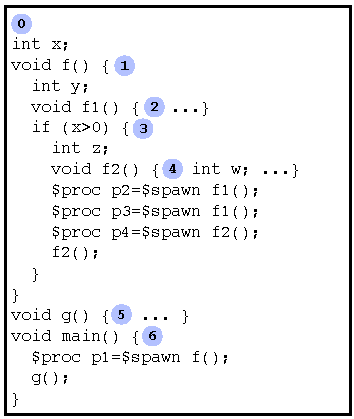
\includegraphics[scale=1.2]{scopeCodeExample}
  \caption{CIVL-C code skeleton to illustrate scope hierarchy}
  \label{fig:scopecodeex}
\end{figure}

\begin{figure}
  \centering
  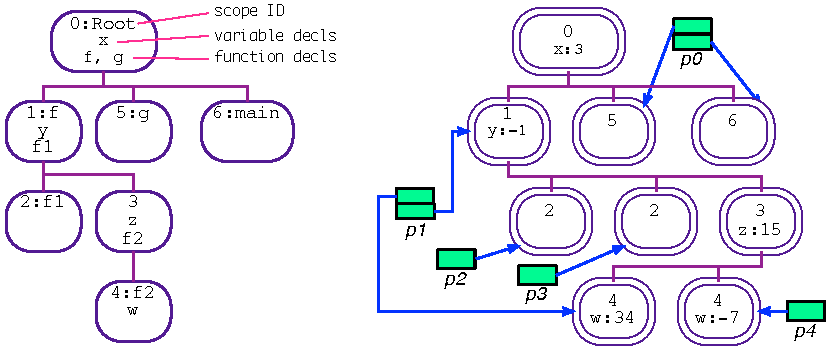
\includegraphics[scale=1.2]{scopeStateExample}
  \caption{Static scope tree and a state for example program}
  \label{fig:scopestateex}
\end{figure}

The static scopes have a tree structure: one scope is a child of
another if the first is immediately contained in the second.  Scope 0,
which is the file scope (or \emph{root} scope) is the root of this
tree.  The static scope tree is depicted in Figure
\ref{fig:scopestateex} (left).  Each scope is identified by its
integer ID.  Additionally, if the scope happens to be the scope of a
function definition, the name of the function is included in this
identifier.  A node in this tree also shows the variables and
functions declared in the scope.  For brevity, we omit the \emph{proc}
variables.

We now look at what happens when this program executes.  Figure
\ref{fig:scopestateex} (right) illustrates a possible state of the
program at one point in an execution.  We now explain how
this state is arrived at.

First, there is an implicit \emph{root function} placed around the
entire code.  The body of the \emph{main} function becomes the body
of the root function, and the \emph{main} function itself disappears.
This minor transformation does not change the structure of the scope
tree.

Execution begins by spawning a process $p_0$ to execute the root
function.  This causes scope $0$ to be instantiated.  An instance of a
static scope is known as a \emph{dynamic scope}, or \emph{dyscopes}
for short.  The dynamic scopes are represented by the ovals with
double borders on the right side of Figure \ref{fig:scopestateex}.
Each dyscope specifies a value for every variable declared in the
corresponding static scope.  In this case, the value $3$ has been
assigned to variable \texttt{x}.

The state of process $p_0$ is represented by a \emph{call stack}
(green).  The entries on this stack are \emph{activation frames}.
Each frame contains two data: a reference to a dyscope (indicated by
blue arrows) and a current location (or programmer counter vaule) in
the static scope corresponding to that dyscope (not shown).  The
dyscope defines the environment in which the process evaluates
expressions and executes statements.  The currently executing function
of a process, corresponding to the top frame in the call stack, can
``see'' only the variables in its dyscope and those of all the
ancestors of its dyscope in the dyscope tree.

Returning to the example, $p_0$ enters scope 6, instanitating that
scope, and then spawns procedure \texttt{f}.  This creates process
$p_1$, with a new stack with a frame pointing to a dyscope
corresponding to static scope 1.  The new process proceed to run
concurrently with $p_0$.  Meanwhile, $p_0$ calls procedure \texttt{g},
which pushes a new entry onto its call stack, and instantiates scope
5.  Hence $p_0$ has two entries on its stack: the bottom one pointing
to the instance of scope 6, the top one pointing to the instance of
scope 5.

Meanwhile, assume $\texttt{x}>0$, so that $p_1$ takes the \emph{true}
branch of the \texttt{if} statement, instantiating scope 3 under the
instance of scope 1.  It then spawns two copies of procedure
\texttt{f1}, creating processes $p_2$ and $p_3$ and two instances of
scope 2.  Then $p_1$ spawns \texttt{f2}, creating process $p_4$ and an
instance of scope 4.  Note that the instance of scope 4 is a chile of
the instance of scope 3, since the (static) scope 4 is a child of
scope 3.  Finally, $p_1$ calls \texttt{f2}, pushing a new entry on its
stack and creating another instance of scope 4.  The final state
arrived at is the one shown.

There are few key points to understand:
\begin{itemize}
\item In any state, there is a mapping from the dyscope tree to the
  static scope tree which maps a dyscope to the static scope of which
  it is an instance.  This mapping is a \emph{tree homomorphism},
  i.e., if dyscope $u$ is a child of dyscope $v$, then the static
  scope corresponding to $u$ is a child of the static scope
  corresponding to $v$.
\item A static scope may have any number of instances, including 0.
\item Dynamic scopes are created when control enters the corresponding
  static scope; they disappear from the state when they become
  unreachable.  A dyscope $v$ is ``reachable'' if some process has a
  frame pointing to a dyscope $u$ and there is a path from $u$ up to
  $v$ that follows the parent edges in the dyscope tree.
\item Processes are created when functions are spawned; they disappear
  from the state when their stack becomes empty (either because the
  process terminates normally or invokes the \emph{exit} system
  function).
\end{itemize}

\section{Structure of a CIVL-C program}

A CIVL-C program is structured very much like a standard C program.
In particular, a CIVL-C program may use the preprocessor directives
specified in the C Standard, and with the same meaning.  A source
program is preprocessed, then parsed, resulting in a translation unit,
just as with standard C.  The main differences are the nesting of
function definitions and the new primitives beginning with
\texttt{\$}, which are described in detail in the remainder of this
part of the manual.

A CIVL-C program must begin with the line
\begin{verbatim}
#include <civlc.h>
\end{verbatim}
which includes the main CIVL-C header file, which declares all the
types and other CIVL primitives.

As usual, a translation unit consists of a sequence of variable
declarations, function prototypes, and function definitions in file
scope.  In addition, \emph{assume} statements may occur in the file
scope.  These are used to state assumptions on the input values
to a program.

\chapter{Sequential Elements}

In this chapter we describe the main sequential elements of the
language.  For the most part these are the same as in C.
Primitives dealing with concurrency are introduced in Chapter
\ref{chap:concurrency}.

\section{Types}

\subsection{Standard types inherited from C}

The boolean type is denoted \verb!_Bool!, as in C. Its values are $0$
and $1$, which are also denoted by $\cfalse$ and $\ctrue$,
respectively.

There is one integer type, corresponding to the mathematical integers.
Currently, all of the C integer types \texttt{int}, \texttt{long},
\texttt{unsigned\ int}, \texttt{short}, etc., are mapped to the CIVL
integer type.

There is one real type, corresponding to the mathematical real
numbers. Currently, all of the C real types \texttt{double},
\texttt{float}, etc., are mapped to the CIVL real type.

Array types, \texttt{struct} and \texttt{union} types, \texttt{char},
and pointer types (including pointers to functions) are all exactly as
in C.

% \subsection{The heap type $\cheap$ and handles}

% Unlike C, a CIVL-C program does not necessarily have access to a
% single, global heap. Instead, there is a $\cheap$ type, and heaps may
% be declared explicitly wherever they are needed. Hence a CIVL-C
% program may have several heaps, and these may exist in different
% scopes.

% A heap is declared and created as follows:
% \begin{verbatim}
%   $heap h = $heap_create();
% \end{verbatim}
% The function \verb!$heap_create()! creates a new empty heap in the
% current scope and returns a \emph{handle} to that heap. A handle is
% like a pointer: it is a reference to another object. However, a handle
% is much more restricted than a general pointer. In particular, it
% cannot be dereferenced (by the \ct{*} operator). The underlying heap
% object can only be accessed by using a handle to it as an argument to
% a system function.

% Handles can be used in assignments and passed as arguments to functions.
% For example, this declaration could follow the one above:
% \begin{verbatim}
%   $heap h2=h;
% \end{verbatim}
% After executing this code, \ct{h2} and \ct{h} will be aliased, i.e., the two
% handles will refer to the same heap object.

% The heap object exists in the scope in which it is created. In
% particular, it will disappear when that scope disappears, i.e., when
% control reaches the right curly brace that defines the end of the
% scope. At that point, any references into the heap become invalid.

% The following system functions deal with heaps:
% \begin{verbatim}
%   void* $malloc($heap h, int size);
%   void free(void *p)
% \end{verbatim}
% The first function is like C's \texttt{malloc}, except that you
% specify the heap in which the allocation takes place.
% This modifies the specified heap and returns a pointer to the new object.
% The function can only occur in a context in which the type of the object is
% specified, as in:
% \begin{verbatim}
%   $heap h;
%   int n = 10;
%   double *p = (double*)$malloc(h, n*sizeof(double));
% \end{verbatim}
% The function \ct{free} is exactly the same as in C. Note that
% \texttt{free} modifies the heap which was used to allocate \texttt{p}.


\subsection{The bundle type: \cbundle}

CIVL-C includes a type named \cbundle. A bundle is basically a
sequence of data, wrapped into an atomic package. A bundle is created
using a function that specifies a region of memory. One can create a
bundle from an array of integers, and another bundle from an array of
reals. Both bundles have the same type, \cbundle. They can therefore
be entered into an array of \cbundle, for example. Hence bundles are
useful for mixing objects of different (even statically unknown) types
into a single data structure. Later, the contents of a bundle can be
extracted with another function that specifies a region of memory into
which to unpack the bundle; if that memory does not have the right
type to receive the contents of the bundle, a runtime error is
generated.

\begin{figure}
\begin{verbatim}
/* Creates a bundle from the memory region specified by ptr and size,
 * copying the data into the new bundle */
$bundle $bundle_pack(void *ptr, int size);

/* Returns the size (number of bytes) of the bundle */
int $bundle_size($bundle b);

/* Copies the data out of the bundle into the region specified */
void $bundle_unpack($bundle bundle, void *ptr);
\end{verbatim}
  \caption{The \emph{bundle} abstract data type}
  \label{fig:bundle}
\end{figure}

The relevant functions for creating and manipulating bundles
are given in Figure \ref{fig:bundle}.

\subsection{The \cscope{} type}
\label{sec:scopetype}

An object of type $\cscope$ is a reference to a dynamic scope.  It may
be thought of as a ``dynamic scope ID, '' but it is not an integer and
cannot be converted to an integer.  Operations defined on scopes are
discussed in Section \ref{sec:scopeexpr}.

\section{Expressions}

\subsection{Expressions inherited from C}

The following C expressions are included in CIVL: 
\begin{itemize}
\item \emph{constant} expressions
\item \emph{identifier} expressions (\texttt{x})
\item parenthetical expressions (\verb!(e)!)
\item numerical \emph{addition} (\verb!a+b!), \emph{subtraction} (\verb!a-b!),
  \emph{multiplication} (\verb!a*b!), \emph{division} (\verb!a/b!),
  \emph{unary plus} (\verb!+a!), \emph{unary minus} (\verb!-a!),
  \emph{integer division} (\verb!a/b!) and \emph{modulus} (\verb!a%b!),
  all with their ideal mathematical interpretations
\item array \emph{index} expressions (\verb!a[e]!) and struct or union
  \emph{navigation} expressions (\verb!x.f!, \verb!p->f!)
\item \emph{address-of} (\verb!&e!), pointer \emph{dereference} (\verb!*p!),
  pointer \emph{addition} (\verb!p+i!) and \emph{subtraction} (\verb!p-q!)
  expressions
\item relational expressions (\verb!a==b!, \verb~a!=b~, \verb!a>=b!,
  \verb!a<=b!, \verb!a<b!, \verb!a>b!)
\item logical \emph{not} (\verb~!p~), \emph{and} (\verb!p&&q!), and
  \emph{or} (\verb!p||q!)
\item \emph{sizeof} a type (\verb!sizeof(t)!) or expression (\verb!sizeof(e)!)
\item \emph{assignment} expressions (\verb!a=b!, \verb!a+=b!, \verb!a-=b!,
  \verb!a*=b!, \verb!a/=b!, \verb!a%=b!, \verb!a++!, \verb!a--!)
\item function \emph{calls} \verb!f(e1,...,en)!
\item \emph{conditional} expressions (\verb!b ? e : f!).
\item \emph{cast} expressions (\verb!(t)e!)
\end{itemize}

Bit-wise operations are not yet supported.

\subsection{Scope expressions}
\label{sec:scopeexpr}

As mentioned in Section \ref{sec:scopetype}, CIVL-C provides a type
\cscope.  An object of this type is a reference to a dynamic scope.
Several constants, expressions, and functions dealing with the
\cscope{} type are also provided.

The $\cscope$ type is like any other object type.  It may be used as
the element type of an array, a field in a structure or union, and so
on.  Expressions of type $\cscope$ may occur on the left or right-hand
sides of assignments and as arguments in function calls just like any
other expression.  Two different variables of type $\cscope$ may be
aliased, i.e., they may refer to the same dynamic scope.

A dynamic scope $\delta$ is \emph{reachable} if there exists a path
which starts from the dyscope referenced by some frame on the call
stack of a process, follows the parent edges in the dyscope tree, and
terminates in $\delta$.  If a dyscope is not reachable, it can never
become reachable, and it cannot have any effect on the subsequent
execution of the program.

Normally, a dynamic scope will eventually become unreachable.  At some
point after it becomes unreachable, it will be collected in a
garbage-collection-like sweep, and any existing references to that
scope will become \emph{undefined}.  An object of type $\cscope$ is
also undefined before it is initialized.  Any use of an undefined
value is reported as an error by CIVL, so it is important to be sure
that a scope variable is defined before using it.


\subsubsection{Checking if a dyscope is defined: \cscopedefined}

The system function \cscopedefined{} has signature
\begin{verbatim}
  _Bool $scope_defined($scope s);
\end{verbatim}
It returns \emph{true} if the dynamic scope specified by \texttt{s} is
defined, else it returns \emph{false}.

\subsubsection{The constant \chere}

A constant \chere{} exists in every scope.  This constant has
type \cscope{} and refers to the dynamic scope in which it is
contained.  For example,
\begin{verbatim}
  { // scope s
    int *p = (int*)$malloc($here, n*sizeof(int));
  }
\end{verbatim}
allocates an object consisting of $n$ ints in the scope $s$.

\subsubsection{The constant \cscoperoot{}}

There is a global constant \cscoperoot{} of type $\cscope$ which
refers to the root dynamic scope.


\subsubsection{Scope relational operators}

Let $s_1$ and $s_2$ be expressions of type \cscope.  The following are
all CIVL-C expressions of boolean type:
\begin{itemize}
\item $s_1$ \ct{==} $s_2$.  This is \emph{true} iff $s_1$ and $s_2$
  refer to the same dynamic scope.
\item  $s_1$ \ct{!=} $s_2$.  This is \emph{true} iff $s_1$ and $s_2$
  refer to different dynamic scopes.
\item  $s_1$ \ct{<=} $s_2$.  This is \emph{true} iff $s_1$ is equal to
  or a descendant of $s_2$, i.e., $s_1$ is equal to or contained in $s_2$.
\item  $s_1$ \ct{<} $s_2$.  This is \emph{true} iff $s_1$ is a strict 
  descendant of $s_2$, i.e., $s_1$ is contained in $s_2$ and is not
  equal to $s_2$.
\item $s_1$ \ct{>} $s_2$.  This is equivalent to $s_2$ \ct{<} $s_1$.
\item  $s_1$ \ct{>=} $s_2$.  This is equivalent to $s_2$ \ct{<=} $s_1$.
\end{itemize}
If $s_1$ or $s_2$ is undefined in any of these expressions, an error
will be reported.

\subsubsection{Scope parent function \texorpdfstring{\cscopeparent}{\$scope\_parent}}

The system function
\begin{verbatim}
  $scope $scope_parent($scope s);
\end{verbatim}
returns the parent dynamic scope of the dynamic scope referenced by
\ct{s}.  If \ct{s} is the root dynamic scope, it returns the undefined
value of type $\cscope$.

\subsubsection{Lowest Common Ancestor: \ct{+}}

The expression $s_1$ \ct{+} $s_2$, where $s_1$ and $s_2$ are
expressions of type \cscope, evaluates to the lowest common ancestor
of $s_1$ and $s_2$ in the dynamic scope tree. This is the smallest
dynamic scope containing both $s_1$ and $s_2$.

\subsubsection{The \cscopeof{} expression}

Given any left-hand-side expression \ct{expr}, the expression
\begin{verbatim}
  $scopeof(expr)
\end{verbatim}
evaluates to the dynamic scope containing the object specified by
\ct{expr}.

The following example illustrates the semantics of the \cscopeof{}
operator.  All of the assertions hold:
\begin{verbatim}
{
  $scope s1 = $here;
  int x;
  double a[10];

  {
    $scope s2 = $here;
    int *p = &x;
    double *q = &a[4];

    assert($scopeof(x)==s1);
    assert($scopeof(p)==s2);
    assert($scopeof(*p)==s1);
    assert($scopeof(a)==s1);
    assert($scopeof(a[5])==s1);
    assert($scopeof(q)==s2);
    assert($scopeof(*q)==s1);
  }
}  
\end{verbatim}

\section{Statements}

The usual C statements are supported:
\begin{itemize}
\item \emph{no-op} (\ct{;})
\item expression statements (\ct{e;})
\item labeled statements, including \ct{case} and \ct{default} labels
  (\ct{l: s})
\item \emph{for} (\ct{for (init; cond; inc) s}), \emph{while} 
  (\ct{while (cond) s}) and \emph{do} (\ct{do s while (cond)})
  loops
\item compound statements (\lb \ct{s1;s2;} \ldots \rb)
\item \texttt{if} and \verb!if! \ldots \verb!else!
\item \verb!goto!
\item \verb!switch!
\item \verb!break!
\item \verb!continue!
\item \verb!return!
\end{itemize}

\section{Guards and nondeterminism}

\subsection{Guarded commands: \cwhen}

A guarded command is encoded in CIVL-C using a $\cwhen$ statement:
\begin{verbatim}
  $when (expr) stmt;
\end{verbatim}
All statements have a guard, either implicit or explicit.  For most
statements, the guard is \ctrue.  The \cwhen{} statement allows one to
attach an explicit guard to a statement.

When \texttt{expr} is \emph{true}, the statement is enabled, otherwise
it is disabled.  A disabled statement is \emph{blocked}---it will not
be scheduled for execution.  When it is enabled, it may execute by
moving control to the \texttt{stmt} and executing the first atomic
action in the \texttt{stmt}.

If \texttt{stmt} itself has a non-trivial guard, the guard of the
\cwhen{} statement is effectively the conjunction of the \texttt{expr}
and the guard of \texttt{stmt}.

The evaluation of \texttt{expr} and the first atomic action of
\texttt{stmt} effectively occur as a single atomic action.  There is
no guarantee that execution of \texttt{stmt} will continue atomically
if it contains more than one atomic action, i.e., other processes may
be scheduled.

Examples:
\begin{verbatim}
  $when (s>0) s--;
\end{verbatim}
This will block until \texttt{s} is positive and then decrement
\texttt{s}.  The execution of \texttt{s--} is guaranteed to take place
in an environment in which \texttt{s} is positive.

\begin{verbatim}
  $when (s>0) {s--; t++}
\end{verbatim}
The execution of \texttt{s--} must happen when \texttt{s>0}, but
between \texttt{s--} and \texttt{t++}, other processes may execute.

\begin{verbatim}
  $when (s>0) $when (t>0) x=y*t;
\end{verbatim}
This blocks until both \texttt{x} and \texttt{t} are positive then
executes the assignment in that state.  It is equivalent to
\begin{verbatim}
  $when (s>0 && t>0) x=y*t;
\end{verbatim}

\subsection{Nondeterministic selection statement: \cchoose}

A \cchoose{} statement has the form
\begin{verbatim}
  $choose {
    stmt1;
    stmt2;
    ...
    default: stmt
  }
\end{verbatim}
The \texttt{default} clause is optional.

The guards of the statements are evaluated and among those that are
\emph{true}, one is chosen nondeterministically and executed.  If none
are \emph{true} and the \texttt{default} clause is present, it is
chosen.  The \texttt{default} clause will only be selected if all
guards are \emph{false}.  If no \texttt{default} clause is present and
all guards are \emph{false}, the statement blocks.  Hence the implicit
guard of the \cchoose{} statement without a \texttt{default} clause is
the disjunction of the guards of its sub-statements.  The implicit
guard of the \cchoose{} statement with a default clause is
\emph{true}.

Example: this shows how to encode a ``low-level'' CIVL guarded
transition system:

\begin{verbatim}
  l1: $choose {
    $when (x>0) {x--; goto l2;}
    $when (x==0) {y=1; goto l3;}
    default: {z=1; goto l4;}
  }
  l2: $choose {
    ...
  }
  l3: $choose {
    ...
  }
\end{verbatim}


\subsection{Nondeterministic choice of integer:
  \texorpdfstring{\cchooseint}{\$choose\_int}}

The system function \cchooseint{} has the following signature:
\begin{verbatim}
  int $choose_int(int n);
\end{verbatim}
This function takes as input a positive integer \texttt{n} and
nondeterministicaly returns an integer in the range
$[0,\texttt{n}-1]$.


\chapter{Concurrency}
\label{chap:concurrency}

\section{Process creation and management}

\subsection{The process type: \cproc}

This is a primitive object type and functions like any other primitive
C type (e.g., \texttt{int}). An object of this type refers to a
process. It can be thought of as a process ID, but it is not an
integer and cannot be cast to one.  It is analogous to the $\cscope$
type for dynamic scopes.

Certain expressions take an argument of \cproc{} type and some return
something of \cproc{} type.  The operators \verb!==! and \verb~!=~ may
be used with two arguments of type \cproc{} to determine whether the
two arguments refer to the same process.

\subsection{Checking if a process is defined: \cprocdefined}

An object of type \cproc{} is initially undefined, so a use of that
object would result in an error.  One can check whether a \cproc{}
object is defined using the method \cprocdefined:
\begin{verbatim}
  _Bool $proc_defined($proc p);
\end{verbatim}

\subsection{The \emph{self} process constant: \cself}

This is a constant of type \cproc. It can be used wherever an argument
of type \cproc{} is called for. It refers to the process that is
evaluating the expression containing \cself.

\subsection{Spawning a new process: \cspawn}

A \emph{spawn} expression is an expression with side-effects.  It
spawns a new process and returns a reference to the new process, i.e.,
an object of type \cproc.  The syntax is the same as a procedure
invocation with the keyword \cspawn{} inserted in front:
\begin{verbatim}
  $spawn f(expr1, ..., exprn)
\end{verbatim}
Typically the returned value is assigned to a variable, e.g.,
\begin{verbatim}
  $proc p = $spawn f(i);
\end{verbatim}
If the invoked function \texttt{f} returns a value, that value is
simply ignored.

\subsection{Waiting for another process to terminate: \cwait}

The system function $\cwait$ has signature
\begin{verbatim}
  void $wait($proc p);
\end{verbatim}
When invoked, this function will not return until the process
referenced by \ct{p} has terminated. Note that $p$ can be any
expression of type \cproc{}, not just a variable.

\subsection{Terminating a process immediately: \cexit}

This function takes no arguments.  It causes the
calling process to terminate immediately, regardless of the state of
its call stack:
\begin{verbatim}
  void $exit(void);
\end{verbatim}

\section{Atomicity}

\subsection{Atom blocks: \catom} This defines a number of statements
to be executed as a single atomic transition.  An \catom~block has the
following form:
\begin{verbatim}
  $atom {
    stmt1;
    stmt2;
    ...
  }
\end{verbatim}

The statements inside an \catom\ block are to be executed as one
transition. It is required that the execution of the statements in an
\catom\ block satisfy all of the following properties:
\begin{enumerate}
\item \emph{deterministic}: at each step in the execution of the atom
  block, there must be at most one enabled statement;
\item \emph{nonblocking}: at each step in the execution, there must be
  at least one enabled statement, hence, together with (1), there must
  be exactly one enabled statement;
\item \emph{finite}: the execution of the atom block must terminate
  after a finite number of steps; and
\item \emph{isolated}: there are no jumps from outside the atom block
  to inside the atom block, or from inside the atomc block to outside
  of it.
\end{enumerate}

Violations of the \emph{deterministic}, \emph{nonblocking}, or
\emph{isolated} properties will be reported either statically or
dynamically.  If the \emph{finite} property is violated, the
verification may just run forever.

Once the process enters an \catom\ block is said to be \emph{executing
  atomly}.  The process remains executing atomly until it reaches the
terminating right brace of the block.  Hence \emph{executing atomly}
is a dynamic, not static condition.  For example, the block might
contain a function call which takes the process to a point in code
which is not statically contained in an atom block; that process is
nevertheless still executing atomly and is subject to the rules above.
The process only stops executing atomly when that function call
returns and control finally reaches the right curly brace at the end
of the atom block (assuming the block is not contained in another atom
block).

\emph{Note:} \cwait\ statements are not allowed in \catom\ blocks.
The rationale for this is that there is never a way to know for
certain that another process has terminated (until \cwait\ has
returned) so there is never a way to be certain the \cwait\ statement
will not block.  If one does occur in an \catom\ block, an error will
be reported statically (if it can be detected statically) or
dynamically (otherwise).  Note that it is not always possible to
detect this statically because the \catom\ block may contain a
function call, and the function may contain the \cwait\ statement.

\subsection{Atomic blocks: \catomic}

The statements in an \emph{atomic} block will be executed without
other processes interleaving, to the extent possible.  It has the
form:
\begin{verbatim}
  $atomic {
    stmt1;
    stmt2;
    ...
  }
\end{verbatim}
It is essentially a weaker form of \catom.  Unlike \catom, there are
no restrictions on the statements that can go inside an \catomic\
block.  A process executing an \catomic~block will try to execute the
statements without interleaving with other processes, unless it
becomes blocked.  Unlike an \catom, the statements in an atomic block
do not necessarily execute as a single transition; they may be spread
out over multiple transitions.

When no statement is enabled, the execution of the \catomic\ block
will be interrupted.  At this point, other processes are allowed to
execute.  Eventually, if the original process becomes enabled due to
the actions of other processes, it may be scheduled again, in which
case it regains atomicity and continues where it left off.  For
example, after executing the first loop, the process executing the
following code will become blocked at the first \cwait\ statement:
 \begin{verbatim}  
$atomic{
  for(int i = 0; i < 5; i++) p[i] = $spawn foo(i);
  for(int i = 0; i < 5; i++) $wait p[i];
}
\end{verbatim}
Other processes will then execute. Eventually, if the process being
waited on terminates, the original process becomes enabled and may be
scheduled, in which case it regain atomicity, increments \texttt{i}
and proceeds to the next $\cwait$ statement.  This is in fact a common
idiom for spawning and waiting on a set of processes.

A process that enters an $\catomic$ block is said to be
\emph{executing atomically}; it remains executing atomically until it
reaches the closing curly brace.

Both $\catom$ and $\catomic$ blocks can be nested arbitrarily, but
$\catom$ overrides $\catomic$: a process that is executing atomly will
continue executing atomly if it encounters an $\catomic$ statement;
but a process executing atomically that encounters an $\catom$ will
begin executing atomly.

The atomic semantics are defined more precisely as follows: there is a
single global variable called the \emph{atomic lock}. This variable
can either be null (meaning the atomic lock is ``free''), or it can
hold the PID of a process; that process is said to ``hold'' the atomic
lock.  Moreover, each process contains a special integer variable, its
\emph{atomic counter}, which is initially 0.  Every time a process
enters an atomic block, it increments its atomic counter; every time
it exits an atomic block, it decrements its counter.  In order to
increment its counter from $0$ to $1$, it must first wait for the
atomic lock to become free, and then take the lock.  When it
decrements its counter from $1$ to $0$, it releases the atomic lock.
When a process executing atomically becomes blocked, it releases the
lock (without changing the value of its atomic counter).


\section{Message-Passing}

CIVL-C provides a number of additional primitives that can be used to
model message-passing systems.  This part of the language is built in
two layers: the lower layer defines an abstract data type for
representing messages; the higher layer defines an abstract data type
of \emph{communicators} for managing sets of messages being
transferred among some set of processes.

\subsection{Messages: \cmessage}

Messages are similar to bundles, but with some additional meta-data.
The \emph{data} component of the message is the ``contents'' of the
message and is formed and extracted much like a bundle.  The meta-data
consists of an integer identifier for the \emph{source} place of the
message, an integer identifier for the message \emph{destination}
place, and an integer \emph{tag} which can be used by a process to
discriminate among messages for reception.  This is very similar to
MPI.

\begin{figure}
  \begin{small}
\begin{verbatim}
/* creates a new message, copying data from the specified buffer */ 
$message $message_pack(int source, int dest, int tag, void *data, int size);

/* returns the message source */ 
int $message_source($message message);

/* returns the message tag */
int $message_tag($message message);

/* returns the message destination */ 
int $message_dest($message message);

/* returns the message size */ 
int $message_size($message message);

/* transfers message data to buf, throwing exception if message
 * size exceeds specified size */ 
void $message_unpack($message message, void *buf, int size);
\end{verbatim}
  \end{small}
  \caption{The \emph{message} abstract data type}
  \label{fig:message}
\end{figure}

The functions for creating, and extracting information from, messages
are given in Figure \ref{fig:message}.

\subsection{Communicators: \cgcomm{} and \ccomm}
\label{sec:communicators}

CIVL-C defines a \emph{global communicator} type $\cgcomm$ and a
\emph{local communicator} type $\ccomm$. The global communicator is an
abstraction for a ``communication universe'' that stores buffered
messages and perhaps other data.  The local communicator wraps
together a reference to a global communicator and an integer
\emph{place}.  Most of the message-passing commands take a local
communicator as an argument to specify the communication universe used
for that operation and the place from which that operation will be
executed.  The communication universes are isolated from one
another---a message sent on one can never be received using a
different communicator, for example.

The global communicator is the shared object that must be declared in
a scope containing all scopes in which communication in that universe
will take place. It is created by specifying the number of
\emph{places} that will comprise the communicator. A place is an
address to which messages may be sent or where they may be received.
There is not necessarily a one-to-one correspondence between places and
processes: many processes can use the same place.

Local communicators are created (typically in some child scope of the
scope in which the global communicator is declared) by specifying the
gobal communicator to which the local one will be associated and the
place ID. The local communicator will be used in most of the
message-passing functions; it may be thought of as an ordered pair
consisting of a reference to the global communicator and the integer
place ID.  The place ID must be in $[0,\texttt{size}-1]$, where
\texttt{size} is the size of the global communicator.  The place ID
specifies the place in the global communication universe that will be
occupied by the local communicator.  The local communicator handle may
be used by more than one process, but all of those processes will be
viewed as occupying the same place.  Only one call to \ccommcreate{}
may occur for each gcomm-place pair.


Both types ($\cgcomm$ and $\ccomm$) are handle types. When declared
with a call to the corresponding creation function, they create an
object in the specified scope and return a handle to that object. The
object can only be accessed through the specified system functions
that take this handle as an argument.

 %  This local communicator handle will be used as an
 % * argument in most message-passing functions.  The place must be in
 % * [0,size-1] and specifies the place in the global communication universe
 % * that will be occupied by the local communicator.  The local communicator
 % * handle may be used by more than one process, but all of those
 % * processes will be viewed as occupying the same place.
 % * Only one call to $comm_create may occur for each gcomm-place pair.

\begin{figure}
  \begin{small}
\begin{verbatim}
/* Creates a new global communicator object and returns a handle to it.
 * The global communicator will have size communication places.  The
 * global communicator defines a communication "universe" and encompasses
 * message buffers and all other components of the state associated to
 * message-passing.  The new object will be allocated in the given scope. */
$gcomm $gcomm_create($scope s, int size);

void $gcomm_destroy($gcomm gcomm); // Destroys the gcomm

_Bool $gcomm_defined($gcomm gcomm); // Is the gcomm object defined?

/* Creates a new local communicator object and returns a handle to it.
 * The new communicator will be affiliated with the specified global
 * communicator. The new object will be allocated in the given scope. */
$comm $comm_create($scope s, $gcomm gcomm, int place);

void $comm_destroy($comm comm); // Destroys the comm

_Bool $comm_defined($comm comm); // Is the comm object defined?

/* Returns the size (number of places) in the global communicator associated
 * to the given comm. */
int $comm_size($comm comm);

/* Returns the place of the local communicator.  This is the same as the
 * place argument used to create the local communicator. */
int $comm_place($comm comm);

/* Adds the message to the appropriate message queue in the communication
 * universe specified by the comm.  The source of the message must equal
 * the place of the comm. */
void $comm_enqueue($comm comm, $message message);

/* Returns true iff a matching message exists in the communication universe
 * specified by the comm.  A message matches the arguments if the destination
 * of the message is the place of the comm, and the sources and tags match. */
_Bool $comm_probe($comm comm, int source, int tag);

/* Finds the first matching message and returns it without modifying
 * the communication universe.  If no matching message exists, returns a message
 * with source, dest, and tag all negative. */
$message $comm_seek($comm comm, int source, int tag);

/* Finds the first matching message, removes it from the communicator,
 * and returns the message */ 
$message $comm_dequeue($comm comm, int source, int tag);
\end{verbatim}
  \end{small}
  \caption{The \emph{communicator} interface specifies handle 
    types $\cgcomm$ and $\ccomm$ and the functions above}
  \label{fig:comm}
\end{figure}

The communicator interface is given in Figure \ref{fig:comm}.

Certain restrictions are enforced on some relations between the
objects involved in a communication universe.

Fix a \cgcomm{} object.  This object corresponds to a single
communication universe with, say, $n$ places.  At any time, there can
be \emph{at most one} \ccomm{} object associated to a given place.  If
a program attempts to create a \ccomm{} object with the same \cgcomm{}
and place as an earlier created \ccomm{} object, a runtime error will
occur.  In particular, there can be at most $n$ \ccomm{} objects
associated to the \cgcomm.

The relation between processes and \ccomm{} objects is unconstrained.
One process may use any number of \ccomm{} objects.  (Of course, the
process must have access to handles for those \ccomm{} objects.)
Dually, a single \ccomm{} object may be used by any number of
processes; this situation arises naturally when modeling a
multi-threaded MPI program.

\begin{figure}
  \begin{small}
\begin{verbatim}
$gcomm gcomm = $gcomm_create($here, nprocs);
void Process(int rank) {
  $comm comm = $comm_create($here, gcomm, rank);

  void Thread(int tid) {
    ...$comm_enqueue(comm, msg)...
    ...$comm_dequeue(comm, source, tag)...
  }

  for (int i=0; i<nthreads; i++) $spawn Thread(i);
  ...
  $comm_destroy(comm);
}
for (int i=0; i<nprocs; i++) $spawn Process(i);
...
$gcomm_destroy(gcomm);
\end{verbatim}
  \end{small}
  \caption{Code skeleton for model of multithreaded MPI program
    showing placement of global and local communicator objects}
  \label{fig:mpi-threads-comm}
\end{figure}

There is no special status given to the process which creates the
\ccomm{} object of a given place.  Any process which can access a
handle for that \ccomm{} object can use it to send or receive
messages, regardless of whether that process was the one that created
the \ccomm{} object.  However, users should be aware that verification
is likely to be most efficient when variables are declared as locally
as possible, so it is best to declare the \ccomm{} object in the
innermost scope possible.  Figure \ref{fig:mpi-threads-comm}
illustrates an effective way to do this in the context of modeling a
multithreaded MPI program.  In the code skeleton, each thread can
access the local communicator object of its process, but not that of
any other process.

\chapter{Specification}

\section{Overview}

Specification is the means by which one expresses what a program is
supposed to do, i.e., what it means for it to be correct.

There are several specification mechanisms in CIVL-C. First, there are
the default properties: these are generic properties which are checked
by default in any program, and require no additional specification
effort. These properties include absence of deadlocks, division by 0,
illegal pointer dereferences, and out of bounds array indexes.

Many more program-specific properties can be specified using
assertions. CIVL-C has a rich assertion language which extends the
language of boolean-valued C expressions. Assumptions are a
specification dual to assertions in that they restrict the set
of executions on which the assertions are checked.

Functional equivalence is a power specification mechanism. In this
approach, two programs are provided, one playing the role of the
specification, the other the role of the implementation. The
implementation is correct if, for all inputs $x$, it produces the same
output as that produced by the specification on input $x$. In other
words, the two programs define the same function; this is sometimes
known as \emph{input-output equivalence}. In order to take this
approach, one must first have a way to specify what the inputs and
outputs of a programs are; CIVL-C provides special keywords for this.

Procedure contracts are another powerful specification mechanisms.
These typically involve specifying preconditions and postconditions
for a function. The function is correct if, whenever it is called in a
state satisfying the precondition, when it returns the state will
satsify the postcondition. A program is correct if all its functions
satsify their contract.

\section{Input-output signature}

\subsection{Input type qualifier: \cinput}

The declaration of a variable in the root scope may
include the type qualifier \cinput, e.g.,
\begin{verbatim}
  $input int n;
\end{verbatim}
This declares the variable to be an input variable, i.e., one which is
considered to be an input to the program.  Such a variable is
initialized with an arbitrary (unconstrained) value of its type.  When
using symbolic execution to verify a program, such a variable will be
assigned a unique symbolic constant of its type.

In contrast, variables in the root scope which are not input variables
will instead be initialized with the ``undefined'' value.  If an
undefined value is used in some way (such as in an argument to an
operator), an error occurs.

In addition, input variables may only be read, never written to.

Alternatively, it is also possible to specify a particular concrete
initial value for an input variable.  This is done using a command
line argument when verifying or running the program.

Input (and output) variables also play a key role when determining
whether two programs are functionally equivalent.  Two programs are
considered functionally equivalent if, whenever they are given the
same inputs (i.e., corresponding \cinput{} variables are initialized
with the same values) they will produce the same outputs (i.e.,
corresponding \coutput{} variables will end up with the same values at
termination).

\subsection{Output type qualifier: \coutput}

A variable in the root scope may be declared with this type qualifier
to declare it to be an output variable.  Output variables are ``dual''
to input variables.  They may only be written to, never read.  They
are used primarily in functional equivalence checking.

\section{Assertions and assumptions}

\subsection{Assertions: \cassert}

The system function \cassert{} takes an argument of boolean type:
\begin{verbatim}
  void $assert (_Bool expr);
\end{verbatim}
During verification, the assertion is checked.  If it cannot be proved
that it must hold, a violation is reported.

Note that CIVL-C boolean expressions have a richer syntax than C
expressions, and may include universal or existential quantifiers
(see below), and the boolean values  \ctrue{} and \cfalse{}.

The assertion function may take additional optional arguments used to
print a specific message if the assertion is violated.  These
additional arguments are similar in form to those used in C's
\texttt{printf} statement: a format string, followed by some number of
arguments which are evaluated and substituted for successive codes in
the format string.  For example,
\begin{verbatim}
  $assert(x<=B, "x-coordinate %f exceeds bound %f", x, B); 
\end{verbatim}

The C function \texttt{assert}, included in the standard library
\texttt{assert.h}, is identical to \cassert.  Programmers are
free to use either one.


\subsection{Assume statements: \cassume}

As \emph{assume statement} has the form
\begin{verbatim}
  $assume expr;
\end{verbatim}
During verification, the assumed expression is assumed to hold.  If
this leads to a contradiction on some execution, that execution is
simply ignored.  It never reports a violation, it only restricts the
set of possible executions that will be explored by the verification
algorithm.

Like as assertion statement, as assume statement can be used any place
a statement is expected.  In addition, as assume statement can be used
in file scope to place restrictions on the global variables of the
programs.  For example,
\begin{verbatim}
$input int B;
$input int N;
$assume 0<=N && N<=B;
\end{verbatim}
declares \texttt{N} and \texttt{B} to be integer inputs and restricts
consideration to inputs satisfying $0\leq\texttt{N}\leq\texttt{B}$.


\section{Formulas}

A formula is a boolean expression that can be used in an assert
statement, assume statement, procedure contract (below), or invariant.
Any ordinary C boolean expression is a formula. CIVL-C provides some
additional kinds of formulas, described below.

\subsection{Implication: \cimplies}

The binary operation \cimplies{} represents logical implication.
The expression \verb!p=>q! is equivalent to \verb~(!p)||q~.

\subsection{Universal quantifier: \cforall}

The universally qunatified formula has the form
\begin{verbatim}
  $forall { type identifier | restriction} expr
\end{verbatim}
where \verb!type! is a type name (e.g., \texttt{int} or
\texttt{double}), \verb!identifier! is the name of the bound variable,
\verb!restriction! is a boolean expression which expresses some
restriction on the values that the bound variable can take, and
\verb!expr! is a formula.  The universally quantified formula
holds iff for all values assignable to the bound variable
for which the restriction holds, the formula \ct{expr} holds.

A variation on the construct above can be used in the special case
where the bound variable is to range over a finite interval
of integers.  In this case the quantified formula may be written:
\begin{verbatim}
  $forall { type identifier=lower .. upper } expr
\end{verbatim}
where \ct{lower} and \ct{upper} are integer expressions.

\subsection{Existential quantifier: \cexists}

The syntax for existentially quantified expressions is exactly the
same as for universally quantified expressions, with \cexists{} in
place of \cforall{}.

\section{Contracts}

\subsection{Procedure contracts: \crequires{} and \censures{}}
The \crequires{} and \censures{} primitives are used to encode
procedure contracts.  There are optional
elements that may occur in a procedure declaration or definition,
as follows.  For a function prototype:
\begin{verbatim}
  T f(...)
    $requires expr;
    $ensures expr;
  ;
\end{verbatim}
For a function definition:
\begin{verbatim}
  T f(...)
    $requires expr;
    $ensures expr;
  {
    ...
  }
\end{verbatim}
The value \cresult{} may be used in post-conditions to refer
to the result returned by a procedure.

\emph{Status}: parsed, but nothing is currently done with this
information.

\subsection{Loop invariants: \cinvariant}

This indicates a loop invariant.  Each C loop
construct has an optional invariant clause as follows:
\begin{verbatim}
  while (expr) $invariant (expr) stmt
  for (e1; e2; e3) $invariant (expr) stmt
  do stmt while (expr) $invariant (expr) ;
\end{verbatim}
The invariant encodes the claim that if \texttt{expr} holds upon
entering the loop and the loop condition holds, then it will hold
after completion of execution of the loop body.  The invariant is used
by certain verification techniques.

\emph{Status:} parsed, but nothing is currently done with this
information.

\section{Concurrency specification}

\subsection{Remote expressions: \texttt{e@x}}.

These have the form \verb!expr@x! and refer to a variable in another
process, e.g., \verb!procs[i]@x!. This special kind of expression is
used in collective expressions, which are used to formulate collective
assertions and invariants.

The expression \verb!expr! must have \cproc{} type.  The variable
\texttt{x} must be a statically visible variable in the context in
which it is occurs.  When this expression is evaluated, the evaluation
context will be shifted to the process referred to by \texttt{expr}.

\emph{Status}: not implemented.

\subsection{Collective expressions: \ccollective}.  These have the form
\begin{verbatim}
  $collective(proc_expr, int_expr) expr 
\end{verbatim}
This is a collective expression over a set of processes.  The
expression \texttt{proc{\U}expr} yields a pointer to the first element
of an array of \cproc.  The expression \texttt{int{\U}expr} gives the
length of that array, i.e., the number of processes.  Expression
\texttt{expr} is a boolean-valued expression; it may use remote
expressions to refer to variables in the processes specified in the
array.  Example:
\begin{verbatim}
  $proc procs[N];
  ...
  $assert $collective(procs, N) i==procs[(pid+1)%N]@i ;
\end{verbatim}

\emph{Status}: not implemented.

\chapter{Pointers and Heaps}
\label{chap:pointers}

CIVL-C supports pointers, using the same operators with the same
meanings as C (\texttt{\&}, \texttt{*}, pointer arithmetic).  There is
also a heap in every scope, and system functions to allocate and
deallocate objects in the specified scope.

\section{Memory functions: \texttt{memcpy}}

The function \texttt{memcpy} is defined in the standard C library
\texttt{string.h} and works exactly the same in CIVL-C: it copies
data from the region pointed to by \ct{q} to that pointed to by
\ct{p}.  The signature is

\begin{verbatim}
  void memcpy(void *p, void *q, size_t size);
\end{verbatim}

\section{Heaps, \cmalloc{} and \cfree}

As mentioned above, each dynamic scope has an implicit heap on which
objects can be allocated and deallocated dynamically.  To allocate an
object, one first needs a reference to the dynamic scope to be used.
The system function $\cmalloc$ is like C's \texttt{malloc}, but takes
this extra scope argument:
\begin{verbatim}
  void * $malloc($scope scope, int size);
\end{verbatim}
The standard C function
\begin{verbatim}
  void * malloc(int size);
\end{verbatim}
declared in \texttt{stdlib.h}, is equivalent to \verb!$malloc($root, size)!.

The system function \cfree{} is used to deallocate a heap object;
it is just like C's \texttt{free}:
\begin{verbatim}
  void $free(void *p);
\end{verbatim}
An error is generated if the pointer is not one that was returned by
\cmalloc, or if it was already freed.  The standard C function
\texttt{free}, declared in \texttt{stdlib.h} is identical to \cfree.
The two functions are interchangeable.

% \section{Pointer types}

% Given any object type $T$ and a static scope $s$ in a CIVL-C program,
% there is a type \emph{pointer-to-$T$-in-$s$}.  The type is used to
% represent a pointer to a memory location of type $T$ in scope $s$ or a
% descendant of $s$ (i.e., some scope contained in $s$).

% If scope $s_1$ is a descendant of $s_2$ (i.e., $s_1$ is lexically
% contained in $s_2$), the type \emph{pointer-to-$T$-in-$s_1$} is a
% subtype of \emph{pointer-to-$T$-in-$s_2$}.  This means that any
% expression of the first type can be used wherever an object of the
% second type is expected.  In particular, any expression $e$ of the
% subtype can be assigned to a left-hand-side expression of the
% supertype without explicit casts; also $e$ can be used as an argument
% to a function for which the corresponding parameter has the supertype.

% The syntax for denoting this type adheres to the usual C syntax for
% denoting the type \emph{pointer-to-$T$} with the addition of a scope
% parameter within angular brackets immediately following the \texttt{*}
% token.  For example, to declare a variable \texttt{p} of type
% \emph{pointer-to-$T$-in-$s$}, one writes
% \begin{verbatim}
%   int *<s> p;
% \end{verbatim}
% If the scope modifier \texttt{<...>} is absent, the scope is taken to
% be the root scope $s_0$.  The object has type
% \emph{pointer-to-$T$-in-$s_0$}, which is abreviated as
% \emph{pointer-to-$T$}.  In this way, stanard C programs can be
% interpreted as CIVL-C programs.

% \section{Address-of operator}

% The address-of operator \texttt{\&} returns a pointer of the
% appropriate subtype using the innermost scope in which its left-hand-side
% argument is declared.  For example

% \begin{verbatim}
%   {
%     $scope s1 = $here();
%     int x;
%     double a[N];
%     int *<s1> p = &x;
%     double *<s1> q = &a[2];
%   }
% \end{verbatim}
% is correct (in particular, it is type-correct) because \texttt{\&x}
% has type \emph{pointer-to-\texttt{int}-in-\texttt{s1}}, since
% \texttt{s1} is the scope in which \texttt{x} is declared.

% Another pointer example:
% \begin{small}
% \begin{verbatim}
% { $scope s0 = $here();
%   { $scope s1 = $here();
%     double x;
%     { $scope s2 = $here();
%       double y;
%       double *<s1> p;
%       /* p can only point to something in s1 or descendant, for example, s2 */
%       p = &x; // fine
%       p = &y; // fine
%       p = (double*)$malloc(s0, 10*sizeof(double)); // static type error
%     }
%   }
% }
% \end{verbatim}
% \end{small}

% \section{Pointer addition and subtractions}

% If \texttt{e} is an expression of type \emph{pointer-to-$T$-in-$s$}
% and \texttt{i} is an expression of integer type then \texttt{e+i} also
% has type \emph{pointer-to-$T$-in-$s$}.  In other words, pointer
% addition cannot leave the scope of the original pointer.  This
% reflects the fact that every object is contained in one scope, and
% pointer addition cannot leave the object.

% Pointer subtraction is defined on two pointers of the same type, where
% ``same'' includes the scope.  That is checked statically.  As in C, it
% is only defined if the two pointers point to the same object.  In
% CIVL-C, a runtime error will be thrown if they do not point to the
% same object.

% \section{Semantics of scopes and pointer types}

% A variable of type \cscope{} is treated like any other variable.
% It becomes part of the state when the scope in which it is declared
% is instantiated to form a dynamic scope.  The variable is 
% initialized  at that time and its value cannot change.

% Each time a dynamic scope is instantiated, it is assigned a unique ID
% number.  The exactly value of the ID number is not relevant, it just
% has to be distince from any other scope ID number that currently
% exists in the state.  This is the value that is assigned to the scope
% variable.  Therefore, if a static scope contains a scope variable, and
% that scope is instantiated twice to form two distinct dynamic scopes,
% the values assigned to the two variables will be distinct.

% A pointer value is an ordered pair $\langle \delta,r \rangle$, where
% $\delta$ is a dynamic scope ID and $r$ is a reference to a memory
% location in the static scope associated to $\delta$.  (We will define
% the exact form of a reference later.)

% When a dynamic scope is instantiated, each new variable created is
% assigned a \emph{dynamic type}.  This is a refinement of the static
% type associated to the static variable.   Every dynamic type
% is an instance of exactly one static type.  The dynamic
% type of the newly instantiated variable is an instance of the
% static type of the static variable.

% The dynamic pointer types have the form
% \emph{pointer-to-$t$-in-$\delta$}, where $t$ is a dynamic type and
% $\delta$ is a dynamic scope ID.  For a program to be dynamically type
% safe, such a variable should hold only values of the form $\langle
% \delta, r\rangle$.  In particular, the variable should never be
% assigned a value where the dynamic scope component is a different
% instance of the static scope $s$ associated to $\delta$.

% \section{Pointer casts}

% If scope $s_1$ is contained in scope $s_2$, an expression of type
% \emph{pointer-to-$T$-in-$s_1$} can always be cast to
% \emph{pointer-to-$T$-in-$s_2$},
%  because the first is a subtype of the second.  (As described above,
% the cast is unnecessary.)  

% The cast in the other direction is also allowed, but the dynamic type
% safety of that cast will only be checked at runtime.  In particular, a
% runtime error will result if the cast attempts to cast the pointer
% value to a dynamic scope which does not contain (is an ancestor of)
% the dynamic scope component of the pointer value.

% A type \emph{pointer-to-$T_1$-in-$s$} can be cast to a type
% \emph{pointer-to-$T_2$-in-$s$} according to the usual rules of C.  In
% other words, usual casting rules apply as long as you don't change the
% scope.

% \section{Scope-Parameterized Functions}

% Coming soon.  (Parsed, type checked, not currently used otherwise.)

% \section{Scope-Parameterized Type Definitions}

% Coming soon. (Ditto.)

\chapter{Libraries}

Each of the following libraries is at least partially implemented and can
be included in a CIVL-C program:
\begin{itemize}
\item \ct{assert}
  \begin{itemize}
  \item \verb!void assert(_Bool expr);!
  \end{itemize}
\item \ct{math}
  \begin{itemize}
  \item \verb!double sqrt(double x);!
  \item \verb!double ceil(double x);!
  \item \verb!double exp(double x);!
  \end{itemize}
\item \ct{stdlib}
  \begin{itemize}
  \item \verb!size_t!
  \item \verb!void * malloc(size_t size);!
  \item \verb!void free(void * ptr);!
  \end{itemize}
\item \ct{stdbool}
  \begin{itemize}
  \item \verb!true!
  \item \verb!false!
  \end{itemize}
\item \ct{stddef}
  \begin{itemize}
  \item \verb!size_t!
  \item \verb!NULL!
  \end{itemize}
\item \ct{stdio}
  \begin{itemize}
  \item \verb!int printf(const char * restrict format, ...);!
  \end{itemize}
\item \ct{string}
  \begin{itemize}
  \item \verb!size_t!
  \item \verb!NULL!
  \item \verb!void memcpy(void * restrict dst, const void * restrict src, size_t n);!
  \end{itemize}
\end{itemize}

\part{Semantics}
\label{part:semantics}

\chapter{CIVL Model Syntax}

\section{Notation and terminology}
\label{sec:notation}

Let $\B=\{\true,\false\}$ (the set of boolean values).  Let
$\N=\{0,1,2,\ldots\}$ (the set of natural numbers).

Given a node $u$ in a tree, we let $\ancestors(u)$ denote the set of
all ancestors of $u$, including $u$.  We let $\descendants(u)$ denote
the set of all descendants of $u$, including $u$.

For any set $S$, let $S^*$ denote the set of all finite sequences of
elements of $S$.  The length of a sequence $\xi\in S^*$ is denoted
$\len(\xi)$.  

% This is a lie:
% The elements of the sequence are indexed from $0$ to
% $\len(\xi)-1$.

\section{Definition of Context}
\label{sec:context}

\begin{definition}
  A \emph{CIVL type system} is a tuple comprising the following
  components:
  \begin{enumerate}
  \item a set $\Type$ (the set of \emph{types}),
  \item a type $\bool\in\Type$ (the \emph{boolean type}),
  \item a type $\proc\in\Type$ (the \emph{process-reference type}),
  \item a set $\Var$ (the set of all \emph{typed variables}),
  \item a function $\vtype\colon \Var\ra\Type$ (which gives the
    type of each variable),
  \item a set $\Val$ (the set of all \emph{values}),
  \item a function which assigns to each $t\in\Type$ a subset
    $\Val_t\subseteq\Val$ (the set of values of type $t$)
    and which satisfies $\Val_{\bool}=\B$ and $\Val_{\proc}=\N$,
  \item a function which assigns to each $t\in\Type$ a value
    $\default_t\in\Val_t$.
  \end{enumerate}
\end{definition}

The default value will be used to give an initial value to any
variable.  It could represent something like ``an undefined value of
type $t$'' or a reasonable initial value ($0$ for integers, etc.),
depending on the language one is modeling.

\begin{definition}
  Given a CIVL type system, a \emph{valuation} in that system is a
  function $\eta\colon\Var\ra\Val$ with the property that for any
  $v\in\Var$, $\eta(v)\in\Val_{\vtype(v)}$.
\end{definition}

Given a CIVL type system, we let $\Eval$ denote the set of all
valuations in that system.

\begin{definition}
  Given a CIVL type system, A \emph{CIVL expression system} for that
  type system is a tuple comprising the following components:
  \begin{enumerate}
  \item a set $\Expr$ (the set of all \emph{typed expressions} over
    $\Var$),
  \item a function $\etype\colon\Expr\ra\Type$ (giving the type
    of each expression),
  \item a function
    $\eval\colon\Expr\times\Eval\ra\Val$ (the \emph{evaluation
      function}), satisyfing
    \begin{itemize}
    \item for any $e\in\Expr$ and $\eta\in\Eval$,
      $\eval(e,\eta)\in\Val_{\etype(e)}$,
    \end{itemize}
  \item a function which associates to any $V\subseteq\Var$, a
    subset $\Expr(V)\subseteq\Expr$ (the set of
    \emph{expressions which involve only variables in $V$}) satisfying
    the following:
    \begin{itemize}
    \item for any $V\subseteq\Var$ and $\eta,\eta'\in\Eval$, if
      $\eta(v)=\eta'(v)$ for all $v\in V$, then for any $e\in\Expr(V)$,
      $\eval(e,\eta)=\eval(e,\eta')$
    \end{itemize}
  \end{enumerate}
\end{definition}

\begin{definition}
  A \emph{CIVL context} is a CIVL type system together with
  a CIVL expression system for that type system.
\end{definition}

\begin{figure}
  \notationtable
  \caption{Table of Notation Used to Define CIVL Model Syntax}
  \label{fig:notation}
\end{figure}

\section{Lexical scopes}
\label{sec:scopes}

\begin{definition}
  Given a CIVL context $\mathcal{C}$, a \emph{lexical scope system}
  over $\mathcal{C}$ is a tuple 
  \[
  (\Sigma,\rootscope,\sparent,\vars)
  \]
  consisting of
  \begin{enumerate}
  \item a set $\Sigma$ (the set of \emph{static scopes}),
  \item a scope $\rootscope\in\Sigma$ (the  \emph{root scope}),
  \item a function
    $\sparent\colon\Sigma\setminus\{\rootscope\}\rightarrow
    \Sigma$ such that 
    \[\{(\sparent(\sigma),\sigma)\mid \sigma\in\Sigma\setminus\{\rootscope\}\}\]
    gives $\Sigma$ the structure of a rooted tree with root $\rootscope$,
  \item a function $\vars\colon\Sigma\rightarrow 2^{\Var}$ 
    (specifying the variables \emph{declared} in each scope) satisfying
    \begin{itemize}
    \item $\sigma\neq\tau\implies \vars(\sigma)\cap \vars(\tau)=\emptyset$.
    \end{itemize}
  \end{enumerate}
\end{definition}

\begin{definition}
  Given a CIVL context and scope $\sigma\in\Sigma$,
  the set of \emph{visible variables} in $\sigma$
  is $\bigcup_{\sigma'\in\ancestors(\sigma)}\vars(\sigma')$.
\end{definition}

One way this notion will be used: expressions used in a scope $\sigma$
can only involve variables visible in $\sigma$.

\section{Functions}
\label{sec:functions}

Fix a CIVL context $\mathcal{C}$ and lexical scope system
\[\Lambda=(\Sigma,\rootscope,\sparent,\vars)\] over $\mathcal{C}$.

We introduce a new type symbol $\void$, as in C, to use as the return
type for a function that does not return a value.  Let
$\Type'=\Type\cup\{\void\}$.

\begin{definition}
  A \emph{function prototype} for $\Lambda$ is a tuple
  $(\sigma, t, \xi)$  consisting of
  \begin{enumerate}
  \item a scope $\sigma\in\Sigma\setminus\{\rootscope\}$
    (the \emph{function scope}),
  \item a type $t\in\Type'$ (the \emph{return type}),
  \item a finite sequence $\xi=v_1v_2\cdots v_n\in\vars(\sigma)^*$
    consisting of variables declared in the function scope
    (the \emph{formal parameters}).
  \end{enumerate}
\end{definition}

\begin{definition}
  A \emph{CIVL function prototype system} consists of
  \begin{enumerate}
  \item a set $\Func$ (the \emph{function symbols}),
  \item a function which assigns to each $f\in\Func$ a 
    function prototype, denoted
    \[
    (\fscope(f), \returntype(f), \params(f)),
    \]
    and satisfying
    \begin{itemize}
    \item for any $\sigma\in\Sigma$, there is at most
      one $f\in\Func$ such that $\sigma=\fscope(f)$, and
    \end{itemize}
  \item a \emph{root function} $f_0$ with $\fscope(f_0)=\rootscope$
    and which is the only function with root scope.
  \end{enumerate}
\end{definition}


\begin{definition}
  Given a CIVL function prototype system, and function symbol
  $f\in\Func\setminus\{f_0\}$, the \emph{declaration scope} of $f$ is
  the scope $\sigma=\sparent(\fscope(f))$.  We also write \emph{$f$ is
    declared in $\sigma$.}
\end{definition}

Note the root function $f_0$ has no declaration scope.

Just as every scope has a set of visible variables, there is also
a set of visible functions:
\begin{definition} 
  The functions \emph{visible at scope $\sigma$} are
  those declared in $\sigma$ or an ancestor of $\sigma$.
\end{definition}
We will see that the variables and functions visible at $\sigma$ are
the only variables and functions that can be referred to by statements
and expressions used within $\sigma$.

Note that only certain scopes are function scopes.  There can be
additional scopes (intuitively corresponding to block scopes in a
source program).  Every scope, however, must ``belong to'' exactly one
function.  The precise definition is as follows:
\begin{definition}
  \label{def:func}
  Given a CIVL function prototype system, define
  \[
  \func \colon \Sigma \ra \Func 
  \]
  by
  \[
  \func(\sigma)=
  \begin{cases}
    f & \text{if $\sigma=\fscope(f)$ for some $f\in\Func$}\\
    \func(\sparent(\sigma)) & \text{otherwise.}
  \end{cases}
  \]
  We say \emph{$\sigma$ belongs to $f$}  when $\func(\sigma)=f$.
\end{definition}
Note that the recursion in Definition \ref{def:func} must stop as the
root scope belongs to the root function and the scopes form a tree.


\section{Statements}

Fix a CIVL function prototype system.  A \emph{CIVL statement} is
defined to be a tuple of one of the forms described below.
In each case, we give any restritions on the components of the tuple
and a brief intuition on the statement's semantics.  The precise
semantics will be described in \S\ref{sec:semantics}.

\begin{enumerate}
\item $\langle\code{parassign},V_1,V_2,\psi\rangle$
  \begin{itemize}
  \item $V_1,V_2\subseteq\Var$
  \item $\psi\colon V_2\ra\Expr(V_1)$ satisfying
    $\etype(\psi(v))=\vtype(v)$ for all $v\in V_2$
  \item \emph{meaning}: parallel assignment, i.e., the assignment of new
    values to any or all of the variables in $V_2$. For each variable
    in $V_2$ an expression is given which will be evaluated in the old
    state to compute the new value for that variable.  $V_1$ contains
    all the variables that may be used in those expressions.  Hence
    $V_1$ is the ``read set'' and $V_2$ is the ``write set'' for the
    parallel assignment.
  \end{itemize}
\item $\langle\code{assign},v,e\rangle$
  \begin{itemize}
  \item $v\in\Var$, $e\in\Expr$, $\etype(e)=\vtype(v)$
  \item \emph{meaning}: simple assignment: evaluate an expression $e$ and
    assign result to variable $v$.  It is a special case of
    \code{parassign} but is provided for convenience.
  \end{itemize}
\item $\langle\code{call},y,f,e_1,\ldots,e_n\rangle$
  \begin{itemize}
  \item $y\in\Var$, $f\in\Func$, $e_1,\ldots,e_n\in\Expr$
  \item $n=\numparams(f)$
  \item $\etype(e_i)=\vtype(v_i)$, where $\params(f)=v_1\cdots v_n$
  \item $\returntype(f)=\vtype(y)$
  \item \emph{meaning}: evaluate expressions $e_1,\ldots,e_n$; push
    frame on call stack and move control to guarded transition system
    (see \S\ref{sec:gts}) for function $f$; when $f$ returns, pop
    stack and store returned result in $y$
  \end{itemize}
\item $\langle\code{call},f,e_1,\ldots,e_n\rangle$
  \begin{itemize}
  \item $f\in\Func$, $e_1,\ldots,e_n\in\Expr$
  \item $n=\numparams(f)$
  \item $\etype(e_i)=\vtype(v_i)$, where $\params(f)=v_1\cdots v_n$
  \item \emph{meaning}: like above, but return type may be \code{void}
    or returned value could just be ignored
  \end{itemize}
\item $\langle\code{fork},p,f,e_1,\ldots,e_n\rangle$
  \begin{itemize}
  \item $p\in\Var$, $f\in\Func$, $e_1,\ldots,e_n\in\Expr$
  \item $n=\numparams(f)$
  \item $\etype(e_i)=\vtype(v_i)$, where $\params(f)=v_1\cdots v_n$
  \item $\returntype(f)=\void$
  \item $\vtype(p)=\proc$
  \item \emph{meaning}: evaluate expressions $e_1,\ldots,e_n$;
    create new process and invoke function $f$ in it;
    return, immediately, a reference to the new process and store
    that reference in $p$
  \end{itemize}
\item $\langle\code{join},e\rangle$
  \begin{itemize}
  \item $e\in\Expr$
  \item $\etype(e)=\proc$
  \item \emph{meaning}: evaluate $e$ and wait for the referenced process to terminate
  \end{itemize}
\item $\langle\code{return},e\rangle$
  \begin{itemize}
  \item $e\in\Expr$
  \item \emph{meaning}: evaluate $e$, pop the call stack and return
    control, along with the value, to caller
  \end{itemize}
\item $\langle\code{return}\rangle$
  \begin{itemize}
  \item \emph{meaning}: pop the call stack and return control to caller;
    only to be used in functions returning \code{void}
  \end{itemize}
\item $\langle\code{write},e\rangle$
  \begin{itemize}
  \item $e\in\Expr$
  \item \emph{meaning}: evaluate $e$ and send result to output
  \end{itemize}
\item $\langle\code{noop}\rangle$
  \begin{itemize}
  \item \emph{meaning}: does nothing
  \end{itemize}
\item $\langle\code{assert}, e\rangle$
  \begin{itemize}
  \item $e\in\Expr$, $\vtype(e)=\bool$
  \item \emph{meaning}: evaluate $e$; if result is false, stop
    execution and report error
  \end{itemize}
\item  $\langle\code{assume}, e\rangle$
  \begin{itemize}
  \item $e\in\Expr$, $\vtype(e)=\bool$
  \item \emph{meaning}: assume $e$ holds (i.e., if $e$ does not hold,
    the execution sequence is not a real execution)
  \end{itemize}
\end{enumerate}

\section{Remarks}

The system described is sufficiently general to model pointers. There
can be (one or more) pointer types and corresponding values.  The
parallel assignment statement can be used to model statements like
C's \texttt{*p=e;}.  In the worst case (if no information is known
about where \texttt{p} could point), one can let $V_2=\Var$.
Similarly, expressions that involve \texttt{*p} as a right-hand
side subexpression can always take $V_1=\Var$.

Heaps can also be modeled.  A heap type may be defined and a variable
of that type declared.  Expressions to modify and read from the heap
can be defined, as can pointers into the heap.


\section{Transition system representation of functions}
\label{sec:gts}

\begin{definition}
  Given a CIVL function prototype system and $f\in\Func$,
  a \emph{guarded transition system} for $f$ 
  is a tuple $(\Loc,\lscope,\start, T)$, where
  \begin{itemize}
  \item $\Loc$ is a set (the set of \emph{locations}),
  \item $\lscope\colon\Loc\ra\Sigma$ is a function which associates
    to each $l\in\Loc$ a scope $\lscope(l)\in\Sigma$ belonging to $f$,
  \item $\start\in\Loc$ (the \emph{start location}),
  \item $T$ is a set of \emph{guarded transitions}, each of which has
    the form $\langle l,g,s,l'\rangle$, where
    \begin{itemize}
    \item $l,l'\in\Loc$ (the \emph{source} and \emph{target}
      locations)
    \item $g\in\Expr(V)$, where $V$ is the set of variables visible at
      $\lscope(l)$, and $\etype(g)=\bool$ ($g$ is called the
      \emph{guard}),
    \item $s$ is a statment all of whose constituent variables,
      expressions, and function symbols are visible at $\lscope(l)$.
    \end{itemize}
  \end{itemize}
  Furthermore, if the guarded transition system contains a statement
  of the form $\langle\code{return}\rangle$ then
  $\returntype(f)=\void$.  If it contains a statement of the form
  $\langle\code{return},e\rangle$ then
  \[
  \etype(e)=\returntype(f).
  \]
\end{definition}

\begin{definition}
  Given a CIVL prototype system, a \emph{CIVL model} $M$ for that
  system assigns, to each $f\in\Func$, a guarded transition system
  \[(\Loc_f,\lscope_f, \start_f,T_f)\] for $f$.  Moreover, if $f\neq f'$
  then
  $\Loc_f\cap\Loc_{f'}=\emptyset$.
\end{definition}

\begin{definition}
  Given a CIVL model $M$, let $\Loc=\bigcup_{f\in\Func}\Loc_f$.
\end{definition}

\chapter{CIVL Model Semantics}
\label{sec:semantics}

\section{State}
\label{sec:state}

Fix a CIVL model $M$.  Recall that a valuation is a type-respecting
function from $\Var$ to $\Val$.  Given a subset $V\subseteq\Var$ of
variables, we define a \emph{valuation on $V$} to be a type-respecting
function from $V$ to $\Val$.  Let $\Eval(V)$ denote the set of all
valuations on $V$.  Note that $\Eval(\Var)=\Eval$.

\begin{definition}
  \label{def:state}
  A \emph{state} of a CIVL model $M$ is a tuple 
  \[
  s=(\Delta, \droot, \dparent, \static, \deval, P, \stack),
  \]
  where
  \begin{enumerate}
  \item $\Delta$ is a finite set (the set of \emph{dynamic scopes} in
    $s$),
  \item $\droot\in\Delta$ (the \emph{root dynamic scope}),
  \item $\dparent\colon \Delta\setminus\{\droot\}\ra\Delta$
    is a function such that the set 
    \[
    \{(\dparent(\delta),\delta)\mid \delta\in
    \Delta\setminus\{\droot\}\}
    \]
    gives $\Delta$ the structure of a rooted tree with root $\droot$,
    \item $\static\colon\Delta\ra\Sigma$,
  \item $\static(\droot)=\rootscope$ and $\droot$ is the only
    $\delta\in\Delta$ satisfying $\static(\delta)=\rootscope$,
  \item $\static(\dparent(\delta))=\sparent(\static(\delta))$ for any
    $\delta\in\Delta$,
  \item $\deval$ is a function that assigns to each $\delta\in\Delta$
    a valuation $\deval(\delta)\in\Eval(\vars(\static(\delta)))$,
  \item $P$ (the set of \emph{process IDs} in $s$) 
    is a finite subset of $\Val_{\proc}$, and
  \item $\stack\colon P\ra \Frame^*$, where
    \[
    \Frame=\{(\delta,l)\in\Delta\times\Loc\mid\lscope(l)=\static(\delta)\}.
    \]
  \end{enumerate}
  Let $\State$ denote the set of all states of $M$.
\end{definition}

% say entrance and exit from scopes does not have to be "structured".

Remarks:
\begin{enumerate}
\item We will also refer to dynamic scopes as \emph{dyscopes}.
\item The elements of $\Delta$ contain no intrinsic information.
  Instead, all of the information concerning dyscopes is encoded
  in the functions that take elements of $\Delta$ as arguments.  Hence
  we might just as well call the elements of $\Delta$ ``dynamic scope
  IDs'' (just as we call the elements of $P$ ``process IDs'').  One
  could use natural numbers for the dyscopes, just as one does
  for processes.
\item The reason for using some form of ID for dyscopes and
  processes, rather than just incorporating the data in the
  appropriate part of the state, is that both kinds of objects may be
  shared.  There can be several components of the state that refer to
  the same dyscope $d$: e.g., $d$ could have several children,
  each of which has a parent reference to $d$, as well as a reference
  from a frame.  A process can be referred to by any number of
  variables of type $\proc$.
\item If $\sigma=\static(\delta)$, we say that \emph{$\delta$ is an
    instance of $\sigma$} or \emph{$\sigma$ is the static scope
    associated to $\delta$}.  In general, a static scope can have any
  number (including 0) of dynamic instances. The exception is the root
  scope $\rootscope$, which must have exactly one instance ($\droot$).
\item A valuation $\deval(\delta)$ assigns a value to each variable in
  the static scope associated to $\delta$.  The function $\deval$
  thereby encodes the value of all variables ``in scope'' in state
  $s$.
\item The sequence $\stack(p)$ encodes the state of the call stack of
  process $p$.  The elements of the sequence are called
  \emph{activation frames}.  The first frame in the sequence, i.e.,
  the frame in position $0$, is the bottom of the stack; the last
  frame is the top of the stack.
\item  Each frame refers to a dyscope $\delta$ and a
  location in the static scope associated to $\delta$.
\end{enumerate}


\begin{definition}
  A dyscope $\delta\in\Delta$ is a \emph{function node}
  if $\static(\delta)$ is the function scope of some function.
\end{definition}

\begin{definition}
  Given any $\delta\in\Delta$, $\fnode(\delta)\in\Delta$ is defined as
  follows: if $\delta$ is a function node, then
  $\fnode(\delta)=\delta$, else
  $\fnode(\delta)=\fnode(\dparent(\delta))$.  We call $\fnode(\delta)$
  the \emph{function node associated to $\delta$}.
\end{definition}

The relation $\{(\delta,\delta')\mid \fnode(\delta)=\fnode(\delta')\}$
is an equivalence relation $\sim$ on $\Delta$.  Let
$\bar{\Delta}=\Delta/\sim$ and write $[\delta]$ for the equivalence
class containing $\delta$.

The set of activation frames in a state $s$ may be identified with the 
set
\[
AF(s)=\bigcup_{p\in P}\{p\}\times\{0,\ldots,\len(\stack(p))-1\}
\]
Namely, $(p,i)$ corresponds to the $i^{\text{th}}$ entry in the call
stack $\stack(p)$ (where the elements of the stacks are indexed from
$0$).

Define $\Psi\colon AF(s)\ra \bar{\Delta}$ as follows: given $(p,i)$,
let $(\delta,l)$ be the corresponding frame; set $\Psi(p,i)=[\delta]$.

% \begin{definition}
%   A state $s$ is \emph{well-formed} if all of the following hold:
%   \begin{enumerate}
%   \item for any $\delta\in\Delta$, at most one child of $\delta$ is not
%     a function node,
%   \item the function $\Psi$ is a one-to-one correspondence,
%   \item any $\delta$ occurring in the top frame of a call stack
%     is a leaf node.
%   \end{enumerate}
% \end{definition}


\section{Jump protocol}
\label{sec:jump}

% can only jump if \delta is a leaf node.
% also no other frame can point to a dyscope between \delta
% and the dyscope corresponding to the function scope

% in any state, a "region" of the dyscope tree can have at
% most one (exactly one?) stack frame pointing into it.

% a region in a chain of nodes starting from a dyanmic scope corresonding
% to a function scopes and leading down until you reach another
% function scope.

% whenever you have more than one child in the dynamic tree, all but
% 0 or 1 children must be a function scope

% every dyscope is owned by at most one frame

% can a frame point only to a leaf node?  No, but all of its children
% must be function nodes

% to find out which frame owns which dyscopes:

% approach 1: start from a frame.  frame owns the node it points to.
% move up parents until you hit a function scope and stop.
% that is that frame's region.  No other frame can point into its
% region.  Proof: true in initial state, invariant under
% call and fork.

% invariant: every leaf node in the dyscope tree is pointed
% to by the top frame of the call stack of some process

% Define a \emph{well-formed state}:

% every dyscope node has at most one child which is not a function node

% 1-1 correspondence between leaf nodes and top frames of stacks.

% Define regions in the dyscope tree.   (each region contains one
% function node)


\newcommand{\lub}{\sigma_{\upsty{lub}}}

\begin{figure}[t]
  \begin{algorithm}[H]
    \Procedure{$\upsty{jump}(s\colon\State, p\colon\Val_{\proc},
      l'\colon\Loc)\colon\State$}{%
      let $(\Delta, \droot, \dparent, \static, \deval, P, \stack)=s$\;
      let $\delta$ be the dyscope of the last frame on $\stack(p)$\;
      let $\sigma=\static(\delta)$\;
      let $\sigma'=\lscope(l')$\;
      let $\lub$ be the least upper bound of $\sigma$ and
      $\sigma'$ in the tree $\Sigma$\;
      let $m$ be the minimum integer such that
      $\sparent^m(\sigma)=\lub$\;
      let $\delta_{\upsty{lub}}=\dparent^m(\delta)$\;
      let $n$ be the minimum integer such that
      $\sparent^{n}(\sigma')=\lub$\;
      let $\delta_0,\ldots,\delta_{n-1}$ be $n$ distinct objects not in $\Delta$\;
      let
      \( \displaystyle
      \Delta'=\Delta
      \cup     \{ \delta_0,\ldots,\delta_{n-1} \}
      %\setminus \{ \dparent^j(\delta)\mid 0\leq j<m\}
      \)\;
      define $\dparent'\colon\Delta'\setminus\{\droot\}\ra\Delta'$ by
      \(
      \dparent'(\delta')=
      \begin{cases}
        \dparent(\delta') & \text{if $\delta'\in\Delta$}\\
        \delta_{i+1} & \text{if $\delta'=\delta_{i}$ for some $0\leq i<n-1$}\\
        \delta_{\upsty{lub}} & \text{if $n\geq 1$ and $\delta'=\delta_{n-1}$}
      \end{cases}
      \)\;
      define $\static'\colon\Delta'\ra\Sigma$ by
      \(
      \static'(\delta')=
      \begin{cases}
        \static(\delta') & \text{if $\delta'\in\Delta$}\\
        \sparent^i(\sigma') & \text{if $\delta'=\delta_i$ for some $0\leq i<n$}
      \end{cases}
      \)\;
      for $\delta'\in\Delta'$ and $v\in\vars(\static(\delta'))$,
      let
      \(
      \deval'(\delta')(v) =
      \begin{cases}
        \deval(\delta')(v) & \text{if $\delta'\in\Delta$}\\
        \default_t & \text{otherwise}
      \end{cases}
      \)\;
      define $\stack'$ to be the same as $\stack$ except that
      the last frame on $\stack'(p)$ is replaced with
      $(\delta_0,l')$ if $n\geq 1$, or with $(\delta_{\upsty{lub}},l')$
      if $n=0$\;
      let $s'=(\Delta',\droot,\dparent',\static',\deval',P,\stack')$\;
      return the result of removing all unreachable dyscopes from $s'$\;
    }
  \end{algorithm}
  \caption{Jump protocol: how the state changes when control moves
    to a new location within a function.  The procedure may only
    be called if $\func(\sigma)=\func(\sigma')$, i.e., the jump
    is contained within one function.}
  \label{fig:jump}
\end{figure}
  
When control moves from one location to another within a function's
transition system, dyscopes may be added, because you can jump out of
scope nests and into new scope nests. The motivating idea is that you
have to move up the dyscope tree every time you move past a right
curly brace (i.e., leave a scope) and then push on a new scope for
each left curly brace you move past. So there is a sequence of upward
moves followed by a sequence of pushes to get to the new
location. (And either or both sequences could be empty.)  At the end,
if any dyscopes become unreachable, they are removed from the state.

Note however, that we do not assume that scopes are associated to
locations in a nice lexical pattern (or any pattern at all). The
protocol described here works for any arbitrary assignment of scopes
to locations.

The precise protocol is described in Figure \ref{fig:jump}.  The
algorithm shown there takes as input a well-formed state, a process
ID, and a location $l'$ for the function that $p$ is currently in.
Say the current dyscope for $p$ is $\delta$, and $l'$ is in
static scope $\sigma'$. Let $\sigma=\static(\delta)$.  Hence the
current static scope is $\sigma$ and the new static scope will be $\sigma'$.

First, you have to find the \emph{least upper bound} $\lub$ of
$\sigma$ and $\sigma'$ in the static scope tree. (Hence $\lub$ is a
common anecestor of $\sigma$ and $\sigma'$, and if $\sigma''$ is any
common ancestor of $\sigma$ and $\sigma'$ then $\sigma''$ is an
ancestor or equal to $\lub$.)  Note that the least upper bound must
exist since the function scope is a common ancestor of $\sigma$ and
$\sigma'$.  There is a chain of static scopes from $\sigma$ up to
$\lub$ and a corresponding chain
$\delta,\dparent(\delta),\ldots,\dparent^m(\delta)$ in the dynamic
scope tree.  Let $\delta_{\upsty{lub}}=\dparent^m(\delta)$.  This
will become the least upper bound of $\delta$ and the new dynamic
scope corresponding to $\sigma'$ that will be added to the state.

Next you add new dyscopes corresponding to the chain of static
scopes leading from $\lub$ down to $\sigma'$.  The variables in the
new scopes are assigned the default values for their respective types.
The $\dparent$, $\static$, and $\deval$ maps are adjusted
accordingly.  Finally, the stack is modified by replacing the last
activation frame with a frame referring to the (possibly) new dynamic
scope and new location $l'$.

This protocol is executed every time control moves from one location
to another.

Note that in CIVL all jumps stay within a function.  There is no
way to jump from one function to another (without returning).

A small variation is the protocol for moving to the start location of
a function when the function is first pushed on the stack. Since the
start location is not necessarily in the function scope (it may be a
proper descendant of that scope), you have to execute the second half
of the protocol to push a sequence of scopes from the function scope
to the scope of the start location.

\section{Initial State}

The \emph{initial state} for $M$ is obtained by creating one process
(let $P=\{0\}$) and having it call the root function $f_0$. 
Hence start with the state $s$ in which $P=\{0\}$, $\ldots$.
The initial state is $\upsty{jump}(s,0,\start_{f_0})$.

\section{Transitions}

The transitions follow the usual ``interleaving'' semantics. Given a
state $\sigma$, one defines the set of enabled transitions in $\sigma$
as follows. Let $p\in P$. Look at the last frame $(d,l)$ of
$\stack(p)$ (i.e., the top of the call stack), assuming the stack is
nonempty. Look at all guarded transitions emanating from $l$. For each
such transition, evaluate the guard using the valuation formed by
taking the union of the valuations of all ancestors of $d$ (including
$d$). In other words, follow the standard ``lexical scoping'' protocol
to determine the value of any variable that could occur at this point.
Those transitions whose guard evaluates to $\emph{true}$ are enabled.

For each enabled transition, a new state is generated by executing
the transition's statement.  For the most part, the semantics are obvious,
but there are a few details that are a bit subtle.

\section{Calls and Spawns}

Both calls and forks of a function $f$ entail the creation of a new
frame. First, a new dyscope $d$ corresponding to $\fscope(f)$ is
created. To find out where to stick that new scope in the dynamic
scope tree, proceed as follows: begin in the dyscope for the
process invoking the fork or call and start moving up its parent
sequence until you reach the first dyscope $d'$ whose associated
static scope is the defining scope of $f$. (You must reach such a
scope, or else $f$ would not be visible, and the model would have a
syntax error!) Insert $d$ right under $d'$, i.e.,
$\dparent(d)=d'$. This preserves the required correspondence between
static scopes and dyscopes. Now you move to the start location,
using the jump protocol, which may involve the creation of additional
dyscopes under $d$. The new frame references the last dynamic
scope you created, and the location is the start location of $f$.
Variables are given their initial values in all the newly created
dyscopes (however that is done).

All of that is the same whether the statement is a fork or call. The
only difference is what happens next: for a call, the new frame is
pushed onto the calling process' call stack. For a fork, a new process
is ``created'', i.e., you pick a natural number not in $P$ and
add it to $P$, and push the frame onto the new stack.   To be totally
deterministic, you could pick the least natural number not in $P$.

\section{Garbage collection}

In a state $s$, a dyscope is unreachable if there is no path
from a frame in a call stack to that dyscope (following the
$\dparent$ edges).  You can remove all unreachable dyscopes.

If a process has terminated (has empty stack) and \emph{there are no
references to that process} in the state, you can just remove the process
from the state.

In any state, you can renumber the processes (and update the
references accordingly) however you want, to get rid of gaps, put them
in a canonic order, etc.


\part{Tools}
\label{part:tools}

\chapter{Tool Overview}

\section{Symbolic execution}

The tools currently in the CIVL tool kit all use \emph{symbolic
  execution}.  This is a technique in which variables are assigned
symbolic rather than concrete values.  In particular, input variables
are assigned unique \emph{symbolic constants}, which are symbols such
as $X$, $Y$, and so on.  Operations produce symbolic expressions in
those symbols, such as $(X+Y)/2$.

\section{Commands}

Current tools allow one to \emph{run} a CIVL program using random
choice to resolve nondeterministic choices; \emph{verify} a program
using model checking to explore all states of the program; and
\emph{replay} a trace if an error is found.  There are also commands
to show the results just of preprocessing or parsing a file; as these
are basically sub-tasks of the other tasks, they are used mainly for
debugging.

Each tool is launched from the command line by typing ``\texttt{civl}
\textit{cmd} \ldots'', where \textit{cmd} is one of
\begin{itemize}
\item \ct{help} : print usage information
\item \ct{run}  : run the program using random simulation
\item \ct{verify} : verify program
\item \ct{replay} : replay trace for program
\item \ct{parse} : show result of preprocessing and parsing file
\item \ct{preprocess} : show result of preprocessing file only.
\end{itemize}
The additional arguments and options are described below and are also
shown by the \ct{help} command.

A number of properties are checked when running or verifying
a CIVL program.  These include the following:
\begin{itemize}
\item absence of deadlocks
\item absence of assertion violations
\item absence of division or modulus with denominator $0$
\item absence of illegal pointer dereferences
\item absence of out-of-bounds array indexes
\item absence of invalid casts
\item every object is defined (i.e., initialized) before
  it is used.
\end{itemize}


\section{Options}

The following command line options are available:

\newenvironment{optionlist}{\begin{flushleft}}{\end{flushleft}}
\newcommand{\option}[2]{#1\\[0mm]\makebox[5mm]{}#2\\[3mm]}
\newcommand{\booloption}[3]{\option{\ct{-#1} or \ct{-#1=}\textit{boolean}
    (default: \ct{#2})}{#3}}
\newcommand{\intoption}[3]{\option{\ct{-#1=}\textit{integer}
    (default: \ct{#2})}{#3}}
\newcommand{\mapoption}[2]{\option{\ct{-#1}\textit{key}\ct{=}\textit{value}}{#2}}
\newcommand{\stringoption}[3]{\option{\ct{-#1=}\textit{string}
    (default: \ct{#2})}{#3}}

\begin{optionlist}
  \booloption{debug}{false}{debug mode: print very detailed information}
  \booloption{echo}{false}{print the command line}
  \intoption{errorBound}{1}{stop after finding this many errors}
  \booloption{guided}{false}{user guided simulation; applies only to
    run, ignored for all other commands}
  \intoption{id}{0}{ID number of trace to replay}
  \mapoption{input}{initialize input variable \textit{key} to
    \textit{value}}
  \intoption{maxdepth}{2147483647}{bound on search depth}
  \booloption{min}{false}{search for minimal counterexample}
  \stringoption{por}{std}{partial order reduction (por) choices:
    std (standard por) or scp (scoped por)}
  \booloption{random}{varies}{select enabled transitions randomly;
    default for \texttt{run}, ignored for all other commands}
  \booloption{saveStates}{true}{save states during depth-first search}
  \stringoption{seed}{none}{set the random seed; applies only to run}
  \booloption{showModel}{false}{print the model}
  \booloption{showProverQueries}{false}{print theorem prover queries
    only}
  \booloption{showQueries}{false}{print all queries}
  \booloption{showSavedStates}{false}{print saved states only}
  \booloption{showStates}{false}{print all states}
  \booloption{showTransitions}{false}{print transitions}
  \booloption{simplify}{true}{simplify states?}
  \booloption{solve}{false}{try to solve for concrete counterexample}
  \stringoption{sysIncludePath}{}{set the system include path}
  \stringoption{trace}{}{filename of trace to replay}
  \stringoption{userIncludePath}{}{set the user include path}
  \booloption{verbose}{false}{verbose mode}
\end{optionlist}

\section{Errors}
\label{sec:errors}

When a property violation occurs, either in \emph{verification} or
\emph{run} mode, a brief report is written to the screen.  In
addition, a report may be \emph{logged} in the directory
\texttt{CIVLREP}.

The \emph{error bound} parameter determines how many errors can be
encountered before a search terminates.  By default, the error bound
is 1, meaning a search will stop as soon as the first error is found.
The error bound can be set to a higher number on the command line
using option \emph{errorBound}.

When the error bound is greater than one, the CIVL verifier continues
searching after the first error is discovered.  It first attempts to
``recover'' from the error by adding to the path condition a clause
which guarantees that the error cannot happen.  For example, if the
error was caused by a possible division by zero, $x/y$, where $y$ is
an unconstrained real symbolic constant, CIVL will add to the path
condition the predicate $y\neq 0$, and continue the search.  In some
cases, CIVL determines that the modified path condition is
unsatisfiable, in which case the search will back-track in the usual
symbolic execution way.

In addition to the printed reports, errors are logged.  However, CIVL
follows a protocol aimed at limiting the number of reports of errors
which are essentially the same.  This protocol uses a simple
equivalence relation on the set of errors.  Two erroneous states are
considered equivalent if the errors are of the same \emph{kind}
(deadlock, division by zero, illegal pointer dereference, etc.) and
every process is at the same location in both states.  When an error
is encountered, CIVL first checks to see if an earlier equivalent
errors exists in the log.  If so, the lengths of the traces leading to
the two error states are compared.  If the new trace is shorter, the
old log entry is replaced with the new one.  In this way, only the
shortest representative error trace for each equivalence class of
errors is recorded in the log.

A log entry actually entails two things: first, a plain text entry
similar to the one printed to the screen is made in a log file in
\texttt{CIVLREP}.  The name of this file is usually of the form
\texttt{\textit{root}{\U}log.txt}, where \textit{root} is the root of
the original file name, i.e., the substring of the file name that ends
just before the first `\texttt{.}'.  For example, if the file name is
\texttt{diningBad.cvl}, the log file will be named
\texttt{diningBad{\U}log.txt}.  This is a plain text, human-readable
file which summarizes the results of the verification run.

In addition, each saved trace is stored in a separate file in
\texttt{CIVLREP}.  The names of these files have the form
\texttt{\textit{root}{\U}\textit{id}.trace}, where \textit{id} is the
error ID (reported when the error is printed and logged).  This file
is not intended to be human-readable.  It contains a compressed
representation of the trace, including all of the options and
parameter values and choices made a nondeterministic points.  
This file is used by CIVL when replaying an error trace.

As mentioned above, the CIVL \texttt{replay} command is used to play
an earlier-saved error trace.  When more than one trace has been
saved, the \texttt{-id} command line option can be used to specify
which one to play. (The default \emph{id} is 0).

\chapter{Interpreting the Output}

\section{Transitions}

Transitions are printed during trace \texttt{replay}, in the course of
a \texttt{run}, or during verification if option
\emph{showTransitions} is selected.  A typical transition is printed
as follows:

\begin{verbatim}
State 6, proc 0: 
  44->49: LOOP_FALSE_BRANCH at f0:36.18-23 "i < n";
  49->RET: return (init) at f0:37.0-1 "}";
  7->8: i = 0 at f0:42.7-16 "int i = 0";
--> State 74
\end{verbatim}

This means that the transition begins executing from the state with
ID 6, and it is executed by the process with PID 0.  The transition
is executed in a sequence of atomic steps; in this case there the
transition consists of three steps.

Process 0 begins at location 44; this is a static location in the
program graph of a function in the CIVL model.  Details about the
locations can be seen by printing the CIVL model.  In executing the
first step, control moves from location 44 to location 49.  This first
step is an edge in the program graph corresonding to the \emph{false}
branch of a loop condition, i.e., the branch that exits the loop.

The remainder of the line describing the step specifies the part of
the original source code corresponding to this step.  The source code
fragment can be found in file \texttt{f0}.  To save space and avoid
constantly repeating long paths, all the source files involved in a
program are printed once and assigned keys such as \texttt{f0},
\texttt{f1}, etc.  The legend is printed out once at the beginning of
the run; in this case it is simply the following:
\begin{verbatim}
File name list:
f0	: dining.cvl
\end{verbatim}
The source code fragment begins on character 18 of line 36 of
\texttt{f0}, and extends to character 23 of that line.  This range is
inclusive on the left and exclusive on the right, so the total number
of characters in this range is $23-18=5$.  The five characters from
the source code are printed next inside double quotes.  For longer
ranges, this excerpt will be abbreviated using an elipsis.

The second step executes a \emph{return} statement, which results in
popping the top activation frame from process 0's call stack. The
function returning is \texttt{init}.  Since the program counter for
that frame disappears with the execution of this step, there is no
final value for its new location; this is signified using the
pseudo-location \texttt{RET}.

In the new top frame, control is at location 7, and an assignment
statement is executed, moving control to location 8.  With this last
step, the transition ends at State 74.

Between transitions, processes can be renumbered.  Hence a process
with PID 0 in one state, may have a different PID in another state.
The same is true for dynamic scope IDs.  Within a single transition,
however, these numbers will not change.

\section{States}

States are printed typically when a property is violated, at the
initial or final points of a trace replay, or if the option
\emph{showStates}, \emph{showSavedStates}, \emph{verbose}, or
\emph{debug} is selected.

\begin{figure}
  \begin{small}
\begin{verbatim}
State 84
| Path condition
| | true
| Dynamic scopes
| | dyscope 0 (parent=-1, static=0)
| | | reachers = {1,2}
| | | variables
| | | | __atomic_lock_var = process<-1>
| | | | __heap = NULL
| | | | BOUND = 3
| | | | n = 2
| | | | forks = X_s0v4[0:=0, 1:=-1]
| | dyscope 1 (parent=2, static=5)
| | | reachers = {1}
| | | variables
| | | | __heap = NULL
| | | | left = 0
| | | | right = 1
| | dyscope 2 (parent=0, static=1)
| | | reachers = {1}
| | | variables
| | | | id = 0
| | | | __heap = NULL
| | dyscope 3 (parent=4, static=5)
| | | reachers = {2}
| | | variables
| | | | __heap = NULL
| | | | left = 1
| | | | right = 0
| | dyscope 4 (parent=0, static=1)
| | | reachers = {2}
| | | variables
| | | | id = 1
| | | | __heap = NULL
| Process states
| | process 0
| | | atomicCount = 0
| | | call stack
| | process 1
| | | atomicCount = 0
| | | call stack
| | | | Frame[function=dine, location=25, f0:22.32-44 "forks[right]", scope=1]
| | process 2
| | | atomicCount = 0
| | | call stack
| | | | Frame[function=dine, location=33, f0:26.32-44 "forks[right]", scope=3]
\end{verbatim}
  \end{small}
  \caption{Complete print-out of a state}
  \label{fig:state-print}
\end{figure}

A complete print-out of a state can be seen in Figure
\ref{fig:state-print}.  The state is presented in hierarchical way.
At the top-most level of this hierarchy, there are 3 main parts to the
state:
\begin{enumerate}
\item the \emph{path condition}, i.e., the boolea-valued symbolic
  expression used in symbolic execution to keep track of all
  conditions on the input symbols which must hold in order for the
  current path to have been followed;
\item the \emph{dynamic scopes}, and
\item the \emph{process states}.
\end{enumerate}

The dynamic scopes are numbered starting from 0.  This numbering is
arbitrary and is invisible to the program, i.e., there is no way for
the program to obtain its dynamic scope ID.  This allows the verifier
to renumber dynamic scopes at will in order to transform a state into
an equivalence canonical form.

The print-out of each dynamic scope specifies the ID of the dyscope's
parent in the dyscope tree.  (The root dyscope shows $-1$ for the
parent.)  This specifies the complete tree structure of the dyscopes.
Each dyscope is an instance of some static scope; the representation
also shows the ID of this static scope.

The next line in the representation of the dyscope shows a set of
\emph{reachers}.  These are the PIDs of the processes that can
\emph{reach} this dyscope.  A process can reach a dyscope if there is
path in the dyscope tree that starts from a dyscope referenced by a
frame on the process' call stack and follows the parent edges in the
tree.

The \emph{variables} section of the dyscope representation consists of
one line for each variable in the static scope corresponding to the
dyscope.  There are also special hidden variables, such as the heap.
In each case, the value assigned to the variable is shown.  A value of
\texttt{NULL} indicates that the variable is currently undefined.

The process states section consists of one sub-section for each
process currently in the state.  Like the dynamic scopes, the
processes are numbered in some arbitrary way. For each process, the
value of the \emph{atomic count} is given.  This is the nesting depth
of the atomic blocks in which the process is currently located, i.e.,
the number of times the process has entered an atomic block without
exiting the block.

The call stack of the process lists the activation frames on the stack
from top to bottom.  The frame at the top correspond to the function
currently executing in that process.  The name of the function, the
value of the program counter (location), and the source code for that
location, and the dyscope ID for the frame are shown.

\section{Property Violations}

As described in Section \ref{sec:errors}, an error report is printed
whenever CIVL encounters an error. A typical error report appears as
follows:
\begin{small}
\begin{verbatim}
Error 0 encountered at depth 21:
CIVL execution error (kind: DEADLOCK, certainty: PROVEABLE)
A deadlock is possible:
  Path condition: true
  Enabling predicate: false
ProcessState 0: terminated
ProcessState 1: at location 25, f0:21.30-42 "forks[right]"
  Enabling predicate: false
ProcessState 2: at location 25, f0:21.30-42 "forks[right]"
  Enabling predicate: false
at f0:21.30-42 "forks[right]".
\end{verbatim}
\end{small}

The report begins with ``Error 0''.  The errors are numbered in the
order they are discovered in this search; this indicates that this is
the first (0th) error encountered.  The depth refers to the length of
the depth-first search stack when the error was encountered.  In this
case, the depth was 21, meaning that the trace leading to the
erroneous state is a sequence of 21 states and 20 transitions.

The errors are categorized by \emph{kind}.  The error kinds include
\emph{deadlock}, indicating that it is possible no transition is
enabled in the state; \emph{assertion violation}, indicating an
assertion may fail in the state; \emph{division by zero}; and
\emph{out of bounds}, indicating an array index may be out of bounds,
among many more.

In addition to the brief report shown above, most error reports
also include a complete print-out of the state at which the error
occurred.  They will also include additional information specific
to the kind of error.  For example, the deadlock error report shown
above includes the following information:
\begin{itemize}
\item the value of the path condition;
\item the \emph{enabling predicate}, which is the disjunction of the
  guards associated to all transitions departing from the current
  state. This is the predicate that CIVL has found to possibly be
  unsatisfiable under the context of the path condition; and
\item for each process, the current location of the process and the
  enabling predicate for that process, i.e., the disjunction of the
  guards associated to all transitions departing from the current
  state in that process (CIVL has found that all of these may be
  unsatisfiable).
\end{itemize}

Errors are also categorized as to their \emph{certainty}.  CIVL is
\emph{conservative}, meaning that if it not sure a property holds in a
state, it will report it.  This means that it may sometimes raise
\emph{false alarms}, i.e., report a possible error even when none
exists. The certainty measures how certain CIVL is that the error is
real.  The certainty levels, from most to least certain, are as
follows:
\begin{enumerate}
\item \emph{concrete}: this indicates that CIVL has actually found
  concrete
  values for all input variables that are guaranteed to drive the
  execution along the current trace and result in the error;
\item \emph{proveable}: this indicates that a theorem prover (either
  the external one or CIVL's built-in prover) has determined that
  the error is feasible, which includes proving that the path condition
  is satisfiable; however, it has not necessarily found concrete
  values for the inputs;
\item \emph{maybe}: this indicates the prover is not sure whether this
  is an error; this could be due to the incompleteness of the decision
  procecure, or it could be a real error;
\item \emph{none}: probably an internal CIVL error: the theorem prover
  has not said anything.
\end{enumerate}

\section{Statistics}

\begin{itemize}
\item \emph{validCalls}: the number of calls to the CIVL \emph{valid}
  method, used to determine if a first-order formula is valid under
  a given first-order context.   Some of these queries are resolved
  quickly by CIVL; when CIVL cannot resolve the query itself, it
  calls a separate theorem prover (CVC3)
\item \emph{proverCalls}: the number of calls to the separate theorem
  prover's \emph{valid} method
\item \emph{memory}: the total amount of memory, in bytes, consumed by
  the Java virtual machine at the end of the search/run.
\item \emph{time}: the total time, in seconds, used to perform the
  CIVL operation
\item \emph{maxProcs}: the maximum process count achieved, over all states 
  encountered in the search/run
\item \emph{statesInstantiated}: the number of state objects
  instantiated during the course of the verification/run
\item \emph{statesSaved}: the number of states saved in the course
  of a search
\item \emph{statesSeen}: the number of states pushed onto the 
  depth-first search stack in the course of the search; note
  that ``intermediate states'' created in the process of executing
  a transition are not pushed onto the stack, only the final
  state resulting from the transition is pushed
\item \emph{statesMatched}: the number of times a state encountered
  in the depth-first search was found to match a saved state seen
  earlier in the search
\item \emph{steps}: the total number of primitive steps executed
  during the verification/run.  A step is the smallest, atomic,
  unit of execution; each transition is composed of one or more steps.
  This number is a good measure for the total amount of ``work''
  carried out by CIVL
\item \emph{transitions}: the total number of transitions executed
  during the verification/run.  A transition is a coarser unit
  of execution; each transition consists of one or more steps 
  executed from a single process, resulting in a state which is then
  pushed onto the DFS stack.
\end{itemize}
 
\cleardoublepage
\phantomsection
\addcontentsline{toc}{part}{Bibliography}
\bibliographystyle{acm}
\bibliography{civl}
\end{document}
